%%%%%%%%%%%%%%%%%%%%%%%%%%%%%%%%%%%%%%%%%%%%%%%%%%%%%%%%%%%%%%%%%%
% * <matheuzmoraes@gmail.com> 2018-05-07T22:22:10.464Z:
%
% ^.
% The following comments were written in Portuguese, because this 
% template applies only for School of Technology at University 
% of Campinas, Brazil.
%
% Este é um modelo Latex para monografias de Trabalhos de Conclusão 
% de Curso (TCC) na graduação, monografias de Mestrado e Teses de 
% doutorado da Faculdade de Tecnologia (FT) da Universidade 
% Estadual de Campinas (UNICAMP).
%
% Esse modelo e seu respectivo arquivo de classe de documento 
% foram adaptado do modelo de teses e dissertações do 
% Instituto de Computação da UNICAMP.
%
% Autor: André Leon Sampaio Gradvohl, Dr.
% Email:        gradvohl@ft.unicamp.br
% Lattes CV:    http://lattes.cnpq.br/9343261628675642
% 
% Última versão: 25/setembro/2017
%%%%%%%%%%%%%%%%%%%%%%%%%%%%%%%%%%%%%%%%%%%%%%%%%%%%%%%%%%%%%%%%%%
%
% Escolha: Portugues ou Ingles ou Espanhol.
% Para a versão final do texto, acrescente a palavra "Final",
% como na segunda linha abaixo da próxima.
\documentclass[Portugues,Final]{tese-FT}
%\documentclass[Portugues,Final]{tese-FT}
%\documentclass[Ingles]{tese-FT}
%\documentclass[Espanhol,Final]{tese-FT}

% Para acrescentar comentários ao PDF descomente:
\usepackage
%  [pdfauthor={nome do autor},
%   pdftitle={titulo},
%   pdfkeywords={palavra-chave, palavra-chave},
%   pdfproducer={Latex with hyperref},
%   pdfcreator={pdflatex}]
{hyperref}

%Mantenha o pacote a seguir para citações no formato ABNT
\usepackage[alf]{abntex2cite}

%Mantenha o pacote a seguir para incluir a lista de símbolos.
\usepackage{nomencl}
\makenomenclature

%O pacote a seguir gera um dummy text. Elimine a linha quando
% for editar seu texto.
\usepackage{lipsum}

%Para multirow nas tabelas
\usepackage{multirow}

%Habilitar tabelas longas
\usepackage{longtable}

\usepackage{booktabs}
\usepackage{multirow}
\usepackage{siunitx}

\usepackage{subcaption}

%Uso de algoritmos
\usepackage[portuguese, ruled, linesnumbered]{algorithm2e}

% Adicionado para realizar comentários online
% Remova as três linhas a seguir na versão final
\usepackage[colorinlistoftodos,textsize=small,portuguese, textwidth=2.7cm]{todonotes} \setlength{\marginparwidth}{2.7cm} \reversemarginpar
\newcommand{\todoMatheus}[1]{\todo[color=green!40]{#1}}
\usepackage[draft,addedmarkup=uwave,authormarkup=none]{changes}
\definechangesauthor[color=red]{Andre}
\definechangesauthor[color=blue]{Matheus}

\usepackage{amsmath}
\usepackage{amsthm} %Para usar em definições.
\newtheorem{definition}{Definição}[chapter]
\usepackage{amsfonts}

\usepackage{threeparttable}

\begin{document}

% Escolha entre autor ou autora:
\autor{Matheus Bernardelli de Moraes}
%\autora{Nome da Autora}

% Sempre deve haver um título em português:
%\titulo{Avaliação de Algoritmos de Seleção de Atributos Aplicados à Cenários de Mudança de Conceito em Fluxos de Dados Online}
\titulo{Avaliação de Desempenho de Algoritmos de Seleção de Atributos Aplicados à Classificação de Fluxos de Dados com Mudanças de Conceito}

% Se a língua for o inglês ou o espanhol defina:
%\title{The Dissertation or Thesis Title in English or Spanish for FT}

% Escolha entre orientador ou orientadora e inclua os títulos:
\orientador{Prof. Dr. André Leon Sampaio Gradvohl}
%\orientadora{Profa. Dra. Nome da Orientadora}

% Escolha entre coorientador ou coorientadora, se houver, 
% e inclua os títulos:
%\coorientador{Prof. Dr. Eng. Lic. Nome do Co-Orientador}
%\coorientadora{Prof. Dra. Eng. Lic. Nome da Co-Orientadora}

% Escolha entre uma das quatro opções a seguir (comente as demais):
%\bsi         % para Trabalho de Conclusão de Curso em BSI
%\tads       % para Trabalho de Conclusão de Curso em TADS
\qualificacaoMestrado  % Para textos de qualificação de mestrado.
%\qualificacaoDoutorado % Para textos de qualificação de doutorado.
%\mestrado   % para Dissertação de Mestrado em Tecnologia
%\doutorado  % para Tese de Doutorado em Tecnologia

% Se houve cotutela, defina:
%\cotutela{Universidade Nova de Plutão}

%Defina a data da defesa no formato {Dia}{Mês}{Ano}
\datadadefesa{31}{07}{2018}

% Para a versão final defina:
% Repita o nome do Orientador(a) no primeiro avaliador
\avaliadorA{Prof. Dr. André Leon Sampaio Gradvohl}{FT/UNICAMP}
\avaliadorB{Prof. Dr. João Roberto Bertini Junior}{FT/UNICAMP}
\avaliadorC{Profa. Dra.  Gisele Busichia Baioco}{FT/UNICAMP}
%\avaliadorD{Prof. Dr. Quarto Avaliador}{Instituição do quarto avaliador}
%\avaliadorE{Prof. Dr. Quinto Avaliador}{Instituição do quinto avaliador}
%\avaliadorF{Prof. Dr. Sexto Avaliador}{Instituição do sexto avaliador}
%\avaliadorG{Prof. Dr. Sétimo Avaliador}{Instituição do sétimo avaliador}
%\avaliadorH{Prof. Dr. Oitavo Avaliador}{Instituição do oitavo avaliador}


% Para incluir a ficha catalográfica em PDF na versão final, 
% copie o arquivo PDF, descomente e ajuste a linha a seguir:
%\fichacatalografica{arquivo.pdf} 

% Este comando deve ficar aqui:
\paginasiniciais

% Se houver dedicatória, descomente a linha a seguir:
%\prefacesection{Isso é um teste}
%A dedicatória deve ocupar uma única página.
%
%
% Se houver epígrafe, descomente e edite as linhas a seguir:
% \begin{epigrafe}
% {\it
% Vita brevis,\\
% ars longa,\\
% occasio praeceps,\\
% experimentum periculosum,\\
% iudicium difficile.}
%
% \hfill (Hippocrates)
% \end{epigrafe}
%
%
% Agradecimentos ou Acknowledgements ou Agradecimientos
%\prefacesection{Agradecimentos}
%Os agradecimentos devem ocupar uma única página.

% Sempre deve haver um resumo em português:
\begin{resumo}
Cerca de 2,5 Exabyte de dados são gerados diariamente, provenientes de diferentes dispositivos e aplicações. Isso implica que 90\% de todo conteúdo digital existente foi criado apenas nos últimos dois anos. Uma parcela considerável desses dados
é transmitida em tempo real, em grande volume e alta velocidade, e podem possuir informações importantes de serem analisadas o mais rápido possível. Neste sentido, o objetivo da área de Mineração em Fluxos de Dados é fornecer ferramentas e técnicas para extração de conhecimento desses fluxos de dados de modo \textit{online}, 
na medida em que são transmitidos. Uma dessas técnicas, conhecida como Seleção de Atributos, visa reduzir os fluxos de dados a uma parcela menor, removendo atributos irrelevantes e redundantes, porém mantendo a qualidade preditiva dos classificadores. Embora seleção de atributos seja amplamente utilizada em conjuntos de dados estáticos, sua aplicação em fluxos de dados é desafiadora devido à sua natureza evolutiva. Neste trabalho, apresentamos uma avaliação parcial do desempenho de seis algoritmos de seleção de atributos, quando aplicados ao problema de classificação de fluxos de dados, em especial em cenários onde a distribuição probabilística dos dados varia ao longo do tempo, fenômeno conhecido como Mudança de Conceito. Demonstramos que o desempenho de dois dos seis algoritmos é inferior em comparação com a classificação sem seleção de atributos, tanto no tempo de resposta quanto no consumo de memória. Quanto à acurácia, os resultados apontam que a classificação sem seleção de atributos apresenta resultados superiores na maioria dos cenários, embora essa diferença não seja significativa. Cada algoritmo apresentou em um cenário distinto resultados superiores aos demais, apresentando acurácias finais até 14\% maiores. Os experimentos utilizando conjuntos de dados reais e artificiais apontam um potencial para utilização desses métodos por apresentarem maior adaptabilidade em alguns cenários de mudanças de conceito.

%Quanto à acurácia, cada algoritmo apresentou em um cenário distinto resultados superiores aos demais, apresentando acurácias até 14\% maiores. Os experimentos utilizando conjuntos de dados reais e artificiais apontam um potencial para utilização desses métodos.

\end{resumo}


% Sempre deve haver um abstract:
\begin{abstract}
Around 2.5 Exabyte of data are generated every day, coming from different devices and applications. This situation implies that 90\% of all digital content available were created in the past two years. A considerable part of this data, known as Data Streams, is transmitted in real time, at high volumes and high velocities, and can contain valuable information which has to be analyzed as soon as possible. Therefore, the Stream Data Mining field aims to provide tools and techniques to extract knowledge from this data stream online or, in other words, as soon as they are received. One of these techniques, known as Feature Selection, aims to reduce the size of the data streams by removing irrelevant and redundant features while maintaining the predictive power of the classifier. While feature selection is widely used for static datasets, it is challenging when applied to data streams due to its evolving nature. In this work, we present a partial performance evaluation of six feature selection algorithms, when applied to the data streams classification problem, particularly when the data probabilistic distribution change over time. This phenomenon is known as Concept Drift. Here we show that two of the six algorithms show lower performance when compared to classification without feature selection for both response time and memory consumption. Concerning the accuracy, results show that classification without feature selection presents better results in most scenarios, although this difference is not significative. Both algorithms presented more significant results in one distinct scenario each, showing accuracies up to 14\% higher. The experiments using both real and artificial datasets present a potential for using these methods due to their better adaptability in some concept drift situations. 


%Concerning the accuracy, both algorithms presented more significant results in one distinct scenario each, showing accuracies up to 14\% higher. The experiments using both real and artificial datasets show that there is a potential for using these methods.


\end{abstract}

% Se houver um resumo em espanhol, descomente as linhas a seguir:
%\begin{resumen}
% A mesma regra aplica-se.
%\end{resumen}

% A lista de figuras:
\listoffigures

% A lista de tabelas:
\listoftables

% A lista de abreviações e siglas é opcional:
% \prefacesection{Lista de Abreviações e Siglas}

% A lista de símbolos é opcional:
% \prefacesection{Lista de Símbolos}

% Quem usa o pacote nomencl para abreviaturas pode incluir:
\renewcommand{\nomname}{Lista de Abreviações e Siglas}
\printnomenclature[3cm]

% O sumário vem aqui:
\tableofcontents

% E esta linha deve ficar bem aqui:
\fimdaspaginasiniciais

% O corpo da dissertação ou tese começa aqui:
%
% O comando a seguir inclui o arquivo introducao.tex
% que contém o capítulo de Introdução. 
% Detalhe: não precisa incluir a extensão .tex
\chapter{Introdução}\label{chp:Introducao}

Com o avanço tecnológico e a difusão de tecnologias acessíveis para todas as camadas da sociedade, o volume de dados gerados diariamente impressiona. De acordo com \citeonline{Dobre2014}, 2,5 Exabyte de dados são gerados todos os dias. Isso implica que 90\% de todo conteúdo digital existente atualmente foi criado apenas nos últimos dois anos. 
Esse conjunto de dados em constante crescimento, transmitido em altas velocidades e que torna cada vez difícil mais seu armazenamento em bancos de dados tradicionais, é conhecido como \textit{Big Data} \cite{Siddiqa2016}.

Esses dados são provenientes dos mais diversos tipos de dispositivos, sistemas e aplicações. Dispositivos móveis (como telefones celulares e tablets), computadores pessoais, sensores elétricos, roteadores de internet, aparelhos GPS, redes sociais e 
\textit{websites} em geral são apenas alguns exemplos de fontes geradoras de conteúdo.  Além disso, cada um desses itens cria e transmite seus dados em diferentes velocidades e formatos.

Entretanto, nem tudo que é criado e transmitido digitalmente pode ser considerado, de fato, relevante para determinados propósitos. Neste contexto, os dados, que podem ser caracteres, textos, números, imagens, sons, dentre outros, que sozinhos significam pouco ou quase nada para os seres humanos, precisam ser transformados em informação ou conhecimento, ou seja, conteúdo que possa ser compreendido e utilizado na sua totalidade. 

Um processo que permite a extração de conhecimento de grandes volumes de dados é a classificação de dados. Esse procedimento da área de Aprendizado de Máquina consiste na utilização de um modelo, conhecido como classificador, para identificar em qual categoria (também conhecido como classe) um dado pertence. Desse modo, cada dado fará parte de uma determinada classe, permitindo que os dados sejam categorizados de acordo com suas próprias características.

O processo de classificação é realizado em duas etapas: etapa de treinamento (ou aprendizado) e etapa de classificação. No treinamento, um algoritmo de classificação constrói o modelo classificador utilizando um conjunto de dados que contém classes previamente definidas e conhecidas. Como as classes das tuplas são providenciadas na etapa de treinamento, a classificação de dados é considerada uma ferramenta de Aprendizado Supervisionado. Por fim, a etapa de classificação é utilizada para classificar novas tuplas recebidas \cite{Han2006}. 

A classificação supervisionada de dados persistentes, aqueles armazenados
em conjuntos de dados estáticos, completos e previamente conhecidos é tema difundido na literatura. Entretanto, esse cenário tem se tornado cada vez mais obsoleto. A quantidade de sistemas que precisam processar, classificar e analisar dados transmitidos em tempo real, por sua criticidade, necessidade de atuação rápida ou simplesmente pela impossibilidade de armazenamento e consultas posteriores, devido ao grande volume e velocidades de 
transmissão, é cada vez maior. Essa sequência de dados que chegam continuamente aos sistemas para o processamento é chamada de fluxo de dados. São exemplos de aplicações que lidam com fluxos de dados, a análise de tendências em redes sociais, gerenciamento de desastres naturais, gerenciamento de ataques em redes de computadores
e filtragem de \textit{spam}, dentre outros \cite{Gradvohl2014}.

A necessidade de análise em tempo real, aliada à característica inerente dos fluxos de dados de serem potencialmente infinitos, demanda soluções para que ocorra a redução da dimensão desses dados. Com uma dimensionalidade menor, os fluxos podem ser classificados de modo mais rápido, mais eficiente em termos de acurácia -- visto que com uma menor dimensão os modelos tendem a obter um melhor desempenho -- e menos custoso computacionalmente. Uma solução que permite essa redução é a utilização de algoritmos de Seleção de Atributos. Esses algoritmos visam a eliminação de atributos irrelevantes ou redundantes de um determinado conjunto de dados, reduzindo sua dimensionalidade \cite{Barddal2017}.   

Entretanto, a aplicação de seleção de atributos em fluxos de dados não é trivial devido a natureza volátil desses dados. Os fluxos de dados estão sujeitos à um fenômeno conhecido como Mudança de Conceito. Segundo \citeonline{Gama2014}, esse fenômeno corresponde às mudanças na distribuição probabilística dos dados que podem acontecer ao longo do tempo. Essas mudanças podem acontecer de diferentes formas, como mudanças na características gerais ou na relação entre os atributos do conjunto. 

Por exemplo, as estatísticas de consumo dos consumidores de um determinado setor da indústria podem sofrer diferentes alterações dependendo de fatores econômicos externos, que não estão ligados diretamente ao conjunto de dados, mas afetam-no diretamente, como mudanças de leis, inflação, especulações etc. Um outro exemplo se refere à mudanças súbitas dos interesses de compra de ações de uma determinada empresa no mercado financeiro, promovidas por uma especulação. 

Esses fatores podem causar um impacto tão significativo no conjunto de dados que os algoritmos utilizados previamente se tornam obsoletos ou incapazes de lidar com o novo cenário. Sendo assim, um algoritmo de seleção de atributos para fluxos de dados deve ser capaz não só de reduzir a dimensão dos fluxos, mantendo a qualidade preditiva do classificador, como também de se adaptar às mudanças de conceito que possivelmente ocorram nos fluxos.

Já existem alguns algoritmos de seleção de atributos para fluxos de dados na literatura. 
\citeonline{Katakis2005} propõem um modelo para utilização de um algoritmo de seleção de atributos em conjunto com um classificador, de modo que ambos operem de modo incremental, avaliando os fluxos à medida que são recebidos. Já 
\citeonline{Wang2014} apresentam um algoritmo guloso que realiza a seleção de atributos em cenários onde a dimensão total de atributos é desconhecida.

Por sua vez, \citeonline{Carvalho2006} propõem um algoritmo baseado em erros que utiliza um classificador interno para avaliar, através de um sistema de pesos, qual o subconjunto ótimo de atributos. Já \citeonline{Yu2003} definem
um algoritmo que se utiliza dos conceitos de entropia e incerteza simétrica do campo de teoria da informação para avaliar os atributos.

\citeonline{Wu2013} propõe um algoritmo que utiliza critérios de relevância e redundância, classificando os atributos recebidos à partir de um critério interno de relevância, removendo todos aqueles que eventualmente se tornem redundantes. Por fim, \citeonline{Wang2015} apresentam um algoritmo que utiliza análise espectral de grupos, separando em grupos distintos atributos relevantes e não relevantes.

Entretanto, como apontam \citeonline{Ramirez-Gallego2017}, esses algoritmos são adaptações de outros utilizados no aprendizado de conjuntos de dados persistentes. Sendo assim, esses algoritmos não foram construídos especificamente para lidar com fluxos de dados e, consequentemente, com o fenômeno de mudanças de conceito, podendo não apresentar resultados satisfatórios diante desses cenários, principalmente em mudanças recorrentes, ou seja, que acontecem de forma periódica (e.~g. vendas de um determinado produtivo no inverno e caem no verão).

Contudo, nenhum desses algoritmos foi avaliado diante de cenários de mudanças de conceito. Deste modo, há a necessidade de avaliar o desempenho dos algoritmos apresentados quando aplicados na redução de dimensionalidade de fluxos de dados que apresentem variações probabilísticas. Este trabalho apresenta um levantamento e avaliação de desempenho de seis algoritmos de seleção de atributos para fluxos de dados presentes na literatura, em diferentes cenários, utilizando conjuntos de dados reais e artificiais contendo todos os tipos de mudanças de conceito. 

O objetivo é verificar se tais algoritmos mantêm o bom desempenho mesmo quando a distribuição probabilística dos dados é alterada. A hipótese é que o desempenho dos algoritmos será inferior nesses cenários. Após essa avaliação, confirmando-se a hipótese, serão identificadas e oferecidas oportunidades de melhorias e soluções para otimização, contribuindo para a construção de um algoritmo capaz de reduzir a dimensão dos dados, porém mantendo a qualidade e bom desempenho, mesmo em situações onde haja evolução dos dados.


\section{Objetivos}\label{sec:objetivos} 

O objetivo deste trabalho é avaliar o desempenho dos algoritmos de seleção de atributos mais relevantes  em fluxos de dados, diante de diferentes cenários de mudança de conceito. Pretende-se, ao final dessa avaliação, oferecer contribuições e oportunidades de melhorias para o desenvolvimento de um algoritmo capaz de obter um bom desempenho independente de possíveis mudanças na distribuição de probabilidades
dos dados ao longo de sua geração e processamento. Para atingir o objetivo principal deste trabalho, propõe-se os objetivos específicos a seguir:

\begin{itemize}
\item Caracterizar e selecionar bases de dados contendo diferentes tipos de mudança de conceito.
\item Implementar os algoritmos de seleção de atributos selecionados em linguagem Java.
\item Avaliar o desempenho dos algoritmos utilizando as bases de dados selecionadas previamente.
\item Analisar e indicar oportunidades de melhorias, propondo soluções de correção ou
otimização.
\end{itemize}


\section{Estrutura do Texto}\label{sec:estrutura_texto} 

Esse texto está organizado em sete capítulos da seguinte forma:

\begin{itemize}
%[Andre] use os comandos \ref{label} para referenciar capítulos e seções no texto. Já fiz a substituição nos trechos a seguir.
\item O Capítulo~\ref{chp:referencial} apresenta um referencial teórico dos principais conceitos referentes aos Fluxos de Dados, Sistemas de Processamento de Eventos Complexos, Mudanças de Conceito e sobre os algoritmos de Seleção de Atributos.
\item O Capítulo~\ref{chp:levantamento} apresenta um levantamento bibliográfico contendo os principais trabalhos da literatura relacionados ao tema dessa dissertação de mestrado. 
\item O Capítulo~\ref{chp:metodologia} apresenta a metodologia dos experimentos realizados neste trabalho, incluindo a caracterização dos algoritmos e bases de dados selecionadas, as métricas observadas e a configuração do ambiente.
\item Os resultados parciais obtidos são apresentados no Capítulo~\ref{chp:resultados}.
\item O Capítulo~\ref{chp:conclusoes} apresenta as conclusões obtidas até o presente momento.
\item Por fim, o Capítulo~\ref{chp:cronograma} apresenta o cronograma deste trabalho, além de informações pertinentes às disciplinas cursadas ao longo do programa de mestrado.
\end{itemize}

% Com o avanço tecnológico e a difusão de tecnologias acessíveis para todas as camadas da sociedade, o volume de dados gerados diariamente impressiona. De acordo com \cite{Dobre2014}, 2.5 Exabyte de dados são gerados todos os dias. Isso implica que 90\% de todo conteúdo digital existente atualmente foi criado apenas nos últimos dois anos. 
% Esse conjunto de dados em constante crescimento, transmitido em altas velocidades e que torna cada vez difícil seu armazenamento em bancos de dados tradicionais, é conhecido como \textit{Big Data} \cite{Siddiqa2016}. 

% Esses dados são provenientes dos mais diversos tipos de dispositivos, sistemas e aplicações. Dispositivos móveis (como telefones celulares e tablets), computadores pessoais, sensores elétricos, roteadores de internet, aparelhos GPS, redes sociais e 
% \textit{websites} em geral são apenas alguns exemplos de fontes geradoras de conteúdo.  Além disso, cada um desses itens cria e transmite seus dados em diferentes velocidades e formatos.

% Entretanto, nem tudo que é criado e transmitido digitalmente pode ser considerado, de fato, relevante para determinados propósitos. Neste contexto, os dados, que podem ser caracteres, textos, números, imagens, sons, dentre outros, que sozinhos significam pouco ou quase nada para os seres humanos, precisam ser transformados em informação ou conhecimento, ou seja, conteúdo que possa ser compreendido e utilizado de forma plena.

% Diante da necessidade de extrair informação dessa grande quantidade de dados existente, uma área de pesquisa surgiu como uma possível solução, recebendo cada vez mais atenção nos últimos anos. Esse campo, conhecido como Mineração de Dados, é definido como o processo de extração de conhecimento ou informação de grandes conjuntos de dados. Através de técnicas que atuam desde a preparação	dos dados para análise, através de atividades como limpeza e formatação do conjunto, até a efetiva análise e extração de informação, a mineração de dados busca oferecer soluções para que organizações usuários
% possam usufruir desses dados de maneira significativa \cite{Han2006}.

% Os processos que envolvem a mineração de dados, e consequentemente os procedimentos para extração de informação, também são conhecidos como um processo de Aprendizado 
% \textit{Offline}
% \cite{Jankowski2016}, pois assumem que todo o conjunto de dados já é conhecido
% , está disponível. Assim, quaisquer técnicas que necessitem ser aplicadas utilizarão do conjunto em sua totalidade. Além disso, tais técnicas podem ser reaplicadas no mesmo conjunto sempre que for preciso até que o resultado esperado seja atingido. 

% Entretanto, esse cenário tem se tornado cada vez mais obsoleto. A quantidade
% de sistemas que precisam processar e analisar dados transmitidos em tempo real, por sua criticidade, necessidade de atuação rápida ou simplesmente pela impossibilidade de armazenamento e consultas posteriores, devido ao grande volume e velocidades de 
% transmissão, é cada vez maior. 
% Essa sequência de dados que chegam continuamente aos sistemas para o processamento é chamada de fluxo de dados.São exemplos de aplicações que lidam com fluxos de dados, 
% a análise de tendências em redes sociais, gerenciamento de desastres naturais, gerenciamento de ataques em redes de computadores
% e filtragem de \textit{spam}, dentre outros \cite{Gradvohl2014}.

% \todoMatheus{Rever esse parágrafo}Diferente do processo de aprendizado \textit{offline}, o processamento dos 
% fluxos de dados representam um novo cenário dentro da área de mineração de dados: a extração de conhecimento em dados transmitidos em tempo real ou Aprendizado 
% \textit{Online}. Segundo \cite{Ramirez-Gallego2017}, as principais características dos fluxos de dados, que os diferem dos dados utilizados no aprendizado \textit{offline}
% (também conhecidos como Dados Persistentes) são: o conjunto total dos fluxos não é conhecido previamente, pois são transmitidos sequencialmente, um por vez ou em partes delimitadas; as instâncias podem ser transmitidas em tempos completamente diferentes; os fluxos são potencialmente infinitos; cada instância pode ser acessada apenas um número limitado de vezes; as instâncias precisam ser analisadas em um tempo limitado para oferecer uma resposta em tempo real e evitar congestionamento das filas para processamento; e, por fim, as características probabilísticas das instâncias podem mudar ao longo do tempo. Este último fenômeno é conhecido como Mudança de Conceito. 

% A mudança de conceito é a característica mais desafiadora dos fluxos de dados. Segundo \citeonline{Gama2014}, esse fenômeno corresponde às mudanças na distribuição probabilística dos dados que podem acontecer ao longo do tempo. Essas mudanças podem acontecer de diferentes formas, como mudanças na características gerais dos dados ou na relação entre os atributos do conjunto. Por exemplo, as estatísticas de consumo dos consumidores de um determinado setor da indústria podem sofrer diferentes alterações dependendo de fatores econômicos externos, que não estão ligados diretamente ao conjunto de dados, mas afetam-no diretamente, como mudanças de leis, inflação, especulações etc. Esses fatores podem causar um impacto tão significativo no conjunto de dados que os algoritmos utilizados previamente se tornam obsoletos ou incapazes de lidar com o novo cenário.

% Com o objetivo de lidar com todos esses desafios, algumas técnicas podem ser aplicadas para reduzir tanto o tempo, quanto o custo computacional, necessários para extração de conhecimento dos fluxos de dados. Uma dessas técnicas, conhecida como Seleção de Atributos, visa a eliminação de atributos irrelevantes ou redundantes de um determinado conjunto de dados \cite{Barddal2017}. Através dessa eliminação, o processo de extração de conhecimento tende a ser mais rápido, eficiente em termos de acurácia, visto que com um menor quantidade de atributos os modelos tendem a obter um melhor desempenho e menos custoso. 

% No campo de fluxos de dados, já existem alguns algoritmos de seleção de atributos que trabalham de forma \textit{online}. Entretanto, como aponta \cite{Ramirez-Gallego2017}, a maioria deles são adaptações de algoritmos utilizados no aprendizado 
% \textit{offline}. Sendo assim, esses algoritmos \textit{offline} não foram construídos especificamente para lidar com fluxos de dados e o fenômeno de mudanças de conceito, podendo não apresentar resultados satisfatórios diante desses cenários, principalmente em mudanças recorrentes, ou seja, que acontecem de forma periódica (e.g. vendas de um determinado produtivo no inverno e caem no verão).

% Deste modo,primeiramente, os principais algoritmos de seleção de atributos para fluxos de dados devem ser testados e avaliados diante de diferentes cenários de mudança de conceito a fim de verificar sua eficácia. A construção de um único algoritmo que funcione perfeitamente em todos os cenários é improvável. Entretanto, à partir dessa análise, é possível observar pontos chave e oportunidades para melhorias, visando a construção de um algoritmo que funcione adequadamente tanto em fluxos que não possuam mudanças em sua distribuição, quanto aqueles que apresentem um ou mais tipos de mudança de conceito, mantendo a sua eficácia. 

% \section{Objetivos}\label{sec:objetivos} 

% O objetivo deste trabalho é avaliar o desempenho dos algoritmos de seleção de atributos mais relevantes  em fluxos de dados, diante de diferentes cenários de mudança de conceito. Pretende-se, ao final dessa avaliação, oferecer contribuições e oportunidades de melhorias para o desenvolvimento de um algoritmo capaz de obter um bom desempenho independente de possíveis mudanças na distribuição de probabilidades
% dos dados ao longo de sua geração e processamento. Para atingir o objetivo principal deste trabalho, propõe-se os objetivos específicos a seguir:

% \begin{itemize}
% \item Caracterizar e selecionar bases de dados contendo diferentes tipos de mudança de conceito;
% \item Implementar os algoritmos de seleção de atributos selecionados em linguagem Java;
% \item Avaliar o desempenho dos algoritmos utilizando as bases de dados selecionadas previamente.
% \item Analisar e indicar oportunidades de melhorias, propondo soluções de correção e/ou otimização.
% \end{itemize}


% \section{Estrutura do Texto}\label{sec:estrutura_texto} 

% Esse texto está organizado em sete capítulos da seguinte forma:

% \begin{itemize}
% %[Andre] use os comandos \ref{label} para referenciar capítulos e seções no texto. Já fiz a substituição nos trechos a seguir.
% \item O Capítulo~\ref{chp:referencial} apresenta um referencial teórico dos principais conceitos referentes aos Fluxos de Dados, Sistemas de Processamento de Eventos Complexos, Mudanças de Conceito e sobre os algoritmos de Seleção de Atributos.
% \item O Capítulo~\ref{chp:levantamento} apresenta um levantamento bibliográfico contendo os principais trabalhos da literatura relacionados ao tema dessa dissertação de mestrado. 
% \item O Capítulo~\ref{chp:metodologia} apresenta a metodologia dos experimentos realizados neste trabalho, incluindo a caracterização dos algoritmos e bases de dados selecionadas, as métricas observadas e a configuração do ambiente.
% \item Os resultados parciais obtidos são apresentados no Capítulo~\ref{chp:resultados}.
% \item O Capítulo~\ref{chp:conclusoes} apresenta as conclusões obtidas até o presente momento.
% \item Por fim, o Capítulo~\ref{chp:cronograma} apresenta o cronograma deste trabalho, além de informações pertinentes às disciplinas cursadas ao longo do programa de mestrado.
% \end{itemize}

% O comando a seguir inclui o arquivo levantamento.tex
% que contém o capítulo de levantamento bibliográfico. 
% Detalhe: não precisa incluir a extensão .tex
\chapter{Referencial Teórico}\label{chp:referencial}

Esse capítulo apresenta os principais conceitos desse trabalho. Entre esses conceitos destacam-se as definições do que são eventos, de fluxos de dados, de sistemas de processamento de eventos complexos e suas características principais, dos tipos de mudanças de conceito, do funcionamento do processo de aprendizado ou mineração em fluxos de dados. Além disso, inclui-se uma explicação detalhada sobre algoritmos de seleção de atributos e, finalmente, qual teste de hipótese será utilizado para validar os resultados deste trabalho.

\section{Fluxos de Dados}\label{sec:fluxos_dados}

Segundo o Glossário de Processamento de Eventos, desenvolvido e mantido pela \textit{Event Processing Technical Society} (ETS) 
\nomenclature{ETS}{\textit{Event Processing Technica Society}} 
\cite{Luckham2008}, um evento é qualquer acontecimento ou algo que está acontecendo. Por exemplo, uma transação financeira, o pouso de um avião, uma ocorrência natural como um terremoto, uma mudança de registros em um banco de dados, uma ocorrência cultural ou histórica, dentre outros. Um evento complexo é todo evento que represente um conjunto de outros eventos. Entretanto, esses acontecimentos são abstratos e precisam ser codificados em uma linguagem em que os computadores possam processá-los. Entende-se, portanto, que um evento em sistemas para processamento de eventos complexos (\textit{complex event processing systems} -- CEP)
\nomenclature{CEP}{\textit{Complex Event Processing}} 
é qualquer objeto que represente um determinado evento, e.~g. um registro de uma compra, um e-mail de confirmação de uma reserva de passagem aérea, uma mensagem enviada por um sensor elétrico, um documento de seguro médico dentre outros. Essas sequências de eventos, quando transformados em dados e transmitidos para os sistemas CEP, em alta velocidade e em grande volume, são denominados fluxos de dados. 

Um fluxo de dados $S = \{S_1, S_2, \ldots, S_n\}$ pode conter um ou mais eventos $S_i$, representados em tuplas. Cada tupla é composta por diferentes atributos, contendo informações relevantes ao evento que se refere. As características dos fluxos de dados são consideravelmente distintas daquelas encontradas em conjuntos de dados persistentes (\textit{offline}), segundo \citeonline{Ramirez-Gallego2017}. As principais diferenças são apresentadas na Tabela~\ref{tabela_diferencas}.

\begin{table}[!htb]
\centering
\caption[Principais diferenças entre fluxos de dados e dados persistentes]{Principais diferenças entre fluxos de dados e dados persistentes. Adaptadas de \citeonline{Ramirez-Gallego2017}}
\label{tabela_diferencas}
\begin{longtable}[c]{|p{7.5cm}|p{7.5cm}|}
\hline
\textbf{Fluxos de Dados} & \textbf{Dados Persistentes} \\ \hline
   Não são conhecidos previamente, mas disponibilizados sequencialmente  &             O conjunto de dados total é conhecido      \\ \hline
    Podem ser transmitidos em frequências completamente diferentes  &             Todas as tuplas estão presentes no conjunto inicial     \\ \hline
          São potencialmente infinitos  &             Os conjuntos são finitos     \\ \hline
                  Precisam ser analisados em um tempo limitado &            Os conjuntos podem ser acessados quantas vezes forem necessárias      \\ \hline
                  As características probabilísticas dos dados podem sofrer alterações ao longo do tempo &            Uma vez disponibilizados, os dados do conjunto não sofrem nenhum tipo de alteração      \\ \hline

\end{longtable}
\end{table}


Conforme indicado na Tabela ~\ref{tabela_diferencas},
as características dos fluxos não são conhecidas previamente. Os fluxos são
processados e analisados na medida em que chegam ao sistema, de modo sequencial, respeitando a ordem de chegada. Além disso, cada fluxo pode ser transmitido em uma frequência completamente diferente de outro. Embora alguns padrões possam ser encontrados, não é possível definir em que momento cada fluxo é transmitido. 

Como são potencialmente infinitos, à medida que começam a ser transmitidos, não se pode dizer quando o fluxo cessará. Por seu grande volume e alta velocidade, aliado à possibilidade de conterem informações críticas, esses fluxos precisam ser analisados em tempo limitado. Refazer o processamento e análise em fluxos já processados é, na maioria das vezes, inviável. 

Por fim, como principal fator que os diferencia dos dados persistentes, os fluxos de dados podem sofrer alterações em suas características probabilísticas ao longo do tempo
. Esse fenômeno é conhecido como Mudança de Conceito.

\section{Sistemas de Processamento de Eventos Complexos}\label{sec:complex_event}

De acordo com \citeonline{Gradvohl2016}, os sistemas CEP podem ser definidos como sistemas distribuídos de processamento de fluxos de dados, que recebem como entrada uma ou mais sequências de eventos (os fluxos de dados) e produzem uma saída, que também pode ser uma sequência de eventos. Visto que os fluxos de dados podem ser transmitidos por diferentes dispositivos ou aplicações, produzindo e transmitindo dados em tempo real, os sistemas CEP podem ser entendidos como sistemas de processamento \textit{online}. 


Os sistemas CEP são compostos por basicamente dois tipos de componentes: os componentes de \textit{software}, conhecidos como Operadores; e os componentes de \textit{hardware}, definidos como Nós de Processamento, onde os operadores são executados. Cada operador pode estar em apenas um nó de processamento, embora um mesmo nó possa armazenar e executar um ou mais operadores. Esses componentes são organizados para formarem um Grafo Acíclico Dirigido. Esse arranjo de operadores
é conhecido como a topologia de um sistema CEP. A Figura~\ref{fig:topologia} apresenta um exemplo de topologia em sistemas CEP.


\begin{figure}[!htb]
  \centering
    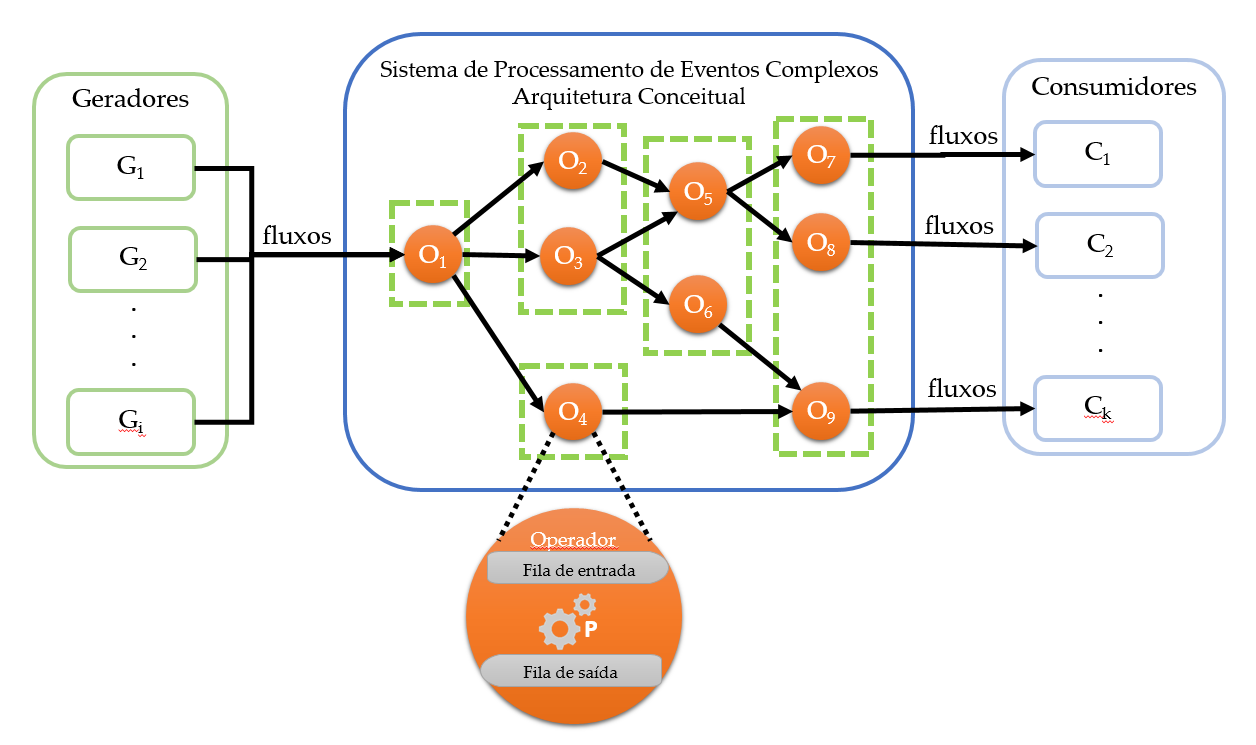
\includegraphics[width=.8\textwidth]{topologia.png}
    \caption{Representação de um sistema CEP, adaptado de \cite{Gradvohl2016}.}
    \label{fig:topologia}
\end{figure}

Conforme ilustra a Figura~\ref{fig:topologia}, dispositivos ou sistemas geradores de conteúdo enviam os dados, em formato de fluxos de dados, para processamento e análise dos sistemas CEP. Quando o fluxo é recebido pelo sistema CEP, suas tuplas são processadas e analisadas pelos operadores pertencentes à sua topologia que, após o processamento, reenviam as tuplas já processadas e analisadas para os demais operadores da topologia, até que todo o ciclo tenha sido finalizado. 

%[Andre] Adicionei uma quebra de parágrafo
Em cada operador, 
a tupla aguardará na fila de entrada até seu efetivo processamento. 
Após o processamento, o operador pode gerar uma nova tupla que será enviada para a fila de saída, 
até seu encaminhamento
para o próximo operador. Por fim, as tuplas são enviadas como fluxos de dados para os Sistemas Consumidores, que receberão os dados processados e analisados, prontos para serem consumidos. 

A etapa mais importante desse processo é o processamento das tuplas por parte dos operadores. Esse processamento pode ser tanto no sentido de analisar os dados recebidos, quanto de aplicar algum algoritmo em cima dos dados, para limpeza, redução ou filtragem, dentre
outras operações.

Em sistemas CEP, os usuários definem \textit{queries} ou regras que especificam como processar os eventos recebidos em formato de fluxos de dados. Conforme aponta \citeonline{Higashino2016}, embora hajam esforços para padronizar as \textit{queries} e garantir uma única linguagem para realização desse processamento, uma grande variedade de linguagens diferentes ainda é utilizada. \citeonline{Margara2011} classificam as linguagens existentes em três grupos distintos:

\begin{itemize}
\item \textbf{Declarativos}: os resultados esperados do processamento são declarados, ao invés de declarar qual fluxo de operadores o processamento deve seguir. Geralmente essas linguagens são derivadas de linguagens relacionais como a álgebra relacional e a SQL.

\item \textbf{Imperativos}: o usuário deve definir um plano para onde cada tupla deve ir e quais operadores deve processá-la. Cada operador transformará as tuplas recebidas em novas tuplas. No geral, os sistemas que trabalham com essa linguagem oferecem ferramentas visuais para definição das regras.

\item \textbf{Baseado em padrões}: linguagens utilizadas para detectar regras nas tuplas recebidas e quais ações devem ser tomadas quando as condições de atuação forem atingidas. Essas condições são definidas geralmente como padrões que são captados pela combinação do uso de operadores lógicos, relacionamentos e constantes de tempo. 
\end{itemize}


Conforme apontado por \citeonline{Higashino2016}, a base para o desenvolvimento dos sistemas CEP se deu à partir do estudo publicado por \citeonline{Luckham1997}.
Nesse estudo, o autor apresenta a ferramenta Rapide, um sistema de simulação para sistemas distribuídos. Por volta do mesmo período, a comunidade científica de banco de dados desenvolveu os primeiros sistemas para processamento de fluxos, como o Aurora \cite{Carney2003} e o STREAM \cite{Arasu2004}. Atualmente, existem diversos sistemas CEP em funcionamento, como o Apache Spark, Apache Storm, Apache Samza, MillWheel dentre outros \cite{Gradvohl2014}.


\section{Mineração em Fluxos de Dados}\label{sec:mineracao_fluxos} 

O método mais comum para extração de conhecimento de fluxos de dados é através do processo de classificação. Essa tarefa é conhecida por categorizar as instâncias de um fluxo de dados entre classes de acordo com suas relações ou afinidades. Assumindo um conjunto de possíveis classes $Y = \{y_1, \ldots, y_c\}$, um classificador constrói um modelo que prevê ou classifica as instâncias ainda não classificadas $\vec{x}_i$ para suas respectivas classes $y_i$.


O processo de classificação pode ser definido formalmente do seguinte modo: um conjunto de $n$ instâncias de treinamento na forma ($\vec{x}_i$, $y_i$) onde $y_i$ é um valor discreto que representa essa classe e $\vec{x}_i$ é um vetor que representa as tuplas, de tamanho $D$-dimensional, onde $D$ representa a quantidade de atributos que essa tupla contém.  Esses atributos podem conter valores categóricos, ordinais, numéricos ou uma representação das três formas. Um classificador é usado para produzir um modelo $f:\vec{x}_i \rightarrow Y$ que classificará as instâncias futuras \cite{Barddal2017}.

De acordo com a Teoria Bayesiana, a classificação pode ser colocada como uma função de probabilidades prévias de uma classe ($P \big[ y \big]$) e a função de densidade de probabilidade condicional ($P \big[ \vec{x} \vert y \big]$) para todas as possíveis classes $y_i \in Y$. A decisão de classificar uma instância em determinada classe é executada de acordo com a probabilidade posterior das classes, onde a Equação ~\ref{eq:bayes} define a probabilidade posterior de uma classe arbitrária $y_i$ e $P  \big[ \vec{x} \big] = \sum_{y_i\in Y} P  \big[ y_i \big] \times P  \big[ \vec{x} \vert y_i \big]$.

\begin{equation}
P  \big[ y_i \vert \vec{x} \big] = \frac{P  \big[ y_i \big] \times P  \big[ \vec{x} \vert y_i \big]}{P  \big[ \vec{x} \big]}	
\label{eq:bayes}
\end{equation}


Tratando-se de mineração em fluxos de dados, são três os principais desafios enfrentados: volume, velocidade e volatilidade. Volatilidade corresponde à um ambiente dinâmico em constante mudança. Volume e velocidade exigem que uma grande massa de dados sejam processado em um tempo limitado. 

%[Andre] Adicionei uma quebra de parágrafo
A princípio, iniciando a partir da primeira tupla recebida, a quantidade de dados aumenta constantemente de zero até potencialmente infinito. Isso exige que sejam utilizadas abordagens que possam se adaptar às mudanças, incorporando informações à medida em que se tornam disponíveis, processando de forma \textit{online} os casos que não possam ser armazenados. Deste modo, para que um algoritmo de mineração em fluxos de dados seja de fato eficiente, é preciso que o mesmo seja adaptável \cite{Krempl2014}.

Segundo 
\citeonline{Gama2010}, 
Algoritmos de Aprendizado Adaptáveis podem ser definidos formalmente do seguinte modo: seja $T_{t} = \{\vec{x}_{i},y_{y} : y = f(\vec{x}) \}$ um conjunto de exemplos disponíveis em um tempo $t \in \{1, 2, 3, \ldots, i\}$. Um algoritmo de aprendizado é adaptável se à partir da sequência de exemplos $\{\ldots, E_{j-1}, E_{j}, \ldots\}$ 
é produzida a sequência de Hipóteses $\{\ldots, H_{j-1}, H_{j}, \ldots\}$ onde cada hipótese $H$ só depende da hipótese anterior $H_{i-1}$ e do exemplo $E_i$. Neste sentido, um algoritmo de aprendizado adaptável requer duas operações: Incremento, quando um exemplo $E_k$ é incorporado no modelo de decisão; e Decremento, quando um exemplo $E_k$ é removido de um modelo de decisão.



\section{Mudanças de Conceito}\label{sec:concept_drift} 

Ao lidar com fluxos de dados, por suas características inerentes, entende-se que serão transmitidos em tempo real, formando um fluxo potencialmente infinito. São inúmeras as possibilidades de distribuição de dados, considerando esse cenário. Espera-se, portanto, que os dados evoluam ao longo do tempo, tornando o ambiente para análise e processamento de fluxos extremamente dinâmico. Essas mudanças ocorrem nos conceitos dos dados do conjunto. A Equação~\ref{eq: conceito} define um conceito C como um conjunto de probabilidades prévias das classes e funções de densidade probabilísticas das classes condicionais, segundo \citeonline{Nguyen2012}.

\begin{equation}
C =   \underset{y\in Y}{\bigcup} \big\{( P\big[ y_i \big],  P\big[ \vec{x} \vert  y_i \big]) \big\}
\label{eq: conceito}
\end{equation}

Portanto, seja $S$ um fluxo de dados com uma quantidade de tuplas $i_t$ com um conceito $C_t$. 
Para todo instante $t_i$ do fluxo, se $C_{t_i} = C_{t_i-1}$, então $C$ é um conceito estável. Caso contrário, se entre dois intervalos de tempo $t_i$ e $t_j = t_i + \Delta \ (\text{ com } \Delta \geq 1)  \ C_{t_i} \neq C_{t_j}$, então uma mudança de conceito aconteceu \cite{Barddal2017}.  
Sendo assim, as probabilidades prévias das classes  $P\big[ y_i \big]$ podem mudar, as probabilidades condicionais das classes $P\big[ \vec{x} \vert  y_i \big]$ podem mudar e as probabilidades posteriores de $P\big[ y_i \vert  \vec{x} \big]$ também podem variar. Essas características afetam a capacidade de classificação dos algoritmos de aprendizado \cite{Gama2014}.

Existem diversas formas em que uma mudança de conceito pode acontecer na distribuição probabilísticas dos dados ao longo do tempo. Desse modo, há várias maneiras de categorizar as mudanças que ocorrem em um conjunto de dados. Uma delas separa as mudanças de conceito por velocidade de mudança, enquanto a outra as divide pelo motivo da mudança \cite{Goncalves2014}. De acordo com \citeonline{Gama2014}, quanto à velocidade de mudança, as categorias são: súbita ou abrupta, incremental, gradual e recorrente. Já a respeito das razões de mudança, as mesmas podem ser reais ou virtuais. 

As razões de mudança são ilustradas na Figura~\ref{fig:razao_mudanca}. Uma mudança real ocorre quando há variações na relação $P\big[ y_i  \vert \vec{x} \big]$, ou seja, quando as tuplas de um fluxo de dados possuem uma legítima classe em determinado momento e outra legítima classe em outro momento. Em contrapartida, uma mudança virtual ocorre quando há mudanças apenas em  $P\big[ \vec{x} \big]$, quando a distribuição dos dados do conjunto (tuplas) é alterada, mas a relação entre os dados e o conceito (classe) permanece o mesmo. No geral, ambas ocorrem de forma conjunta \cite{Goncalves2014}.

\begin{figure}[!htb]
  \centering
    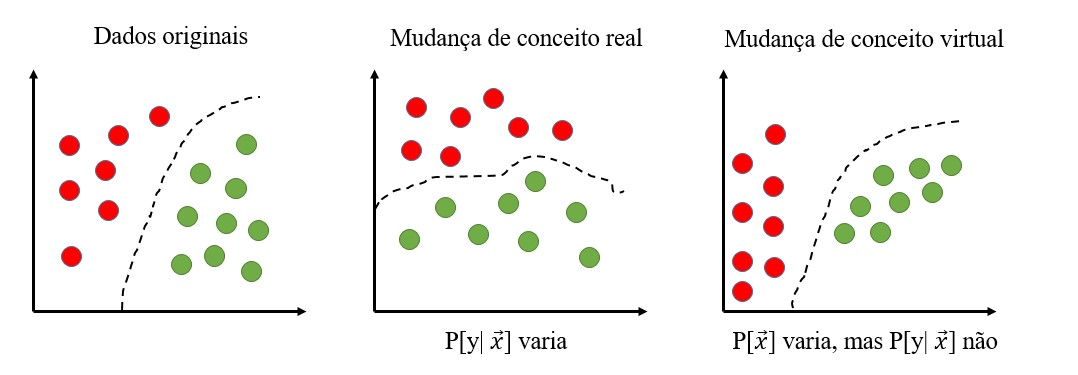
\includegraphics[width=.8\textwidth]{razao_mudanca.jpg}
    \caption[Tipos de mudanças de conceito, em relação à razão de mudança.] %[Andre] Entre colchetes está a legenda resumida. Entre chaves, a legenda completa.
    {Tipos de mudanças de conceito, em relação à razão de mudança. Círculos representam tuplas;  cores diferentes representam classes diferentes. Adaptado de \citeonline{Gama2014}.}
    \label{fig:razao_mudanca}
\end{figure}

O comportamento das mudanças em relação à velocidade de mudança é apresentado na Figura ~\ref{fig:tipos_conceito}. Nesta figura, é dado um exemplo de um conjunto de dados onde o conceito é referente a um atributo média. Conforme ilustrado, uma mudança de conceito súbita ou abrupta ocorre quando os fluxos variam de um conceito para outro repentinamente (e.~g. troca de um sensor por outro que possui uma calibragem diferente).

\begin{figure}[!htb]
  \centering
    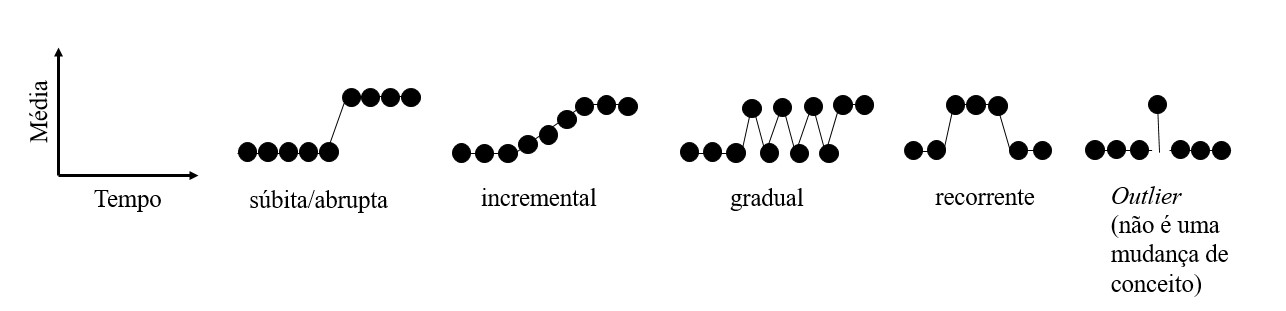
\includegraphics[width=.8\textwidth]{tipos_conceito.jpg}
    \caption[Tipos de mudanças de conceito, em relação à velocidade de mudança.]{Tipos de mudanças de conceito, em relação à velocidade de mudança. Adaptado de \citeonline{Gama2014}.}
    \label{fig:tipos_conceito}
\end{figure}

A mudança pode acontecer incrementalmente, consistindo em vários pontos intermediários dentre dois conceitos consideravelmente distintos (e.~g. um sensor que lentamente se torna menos preciso ao longo do tempo). Há, ainda, a mudança gradual, quando as mudanças não acontecem de forma abrupta, mas continuam voltando ao mesmo padrão antigo por um tempo (e.~g. tópicos de interesse em um jornal para uma pessoa que passará suas férias em outro lugar, onde o indivíduo não mudará repentinamente seus interesses, visualizando os interesses anteriores por um tempo). 

Finalmente, há a mudança recorrente, quando conceitos vistos previamente reaparecem após um intervalo de tempo (e.~g. vendas de um produto sobem no verão e caem no inverno). Por fim, é preciso distinguir a diferença entre mudanças de conceito e \textit{outliers}, que são pontos  que não representam corretamente a distribuição dos dados, podendo ser causados, por exemplo, por algum tipo de erro \cite{Han2006}.

\section{Seleção de Atributos}\label{sec:selecao_atributos} 

A alta dimensionalidade dos conjuntos de dados disponíveis atualmente, com o advento de \textit{Big Data}, representa um grande desafio para extração de conhecimento de grandes volumes de dados. Por exemplo, \citeonline{Weinberger2009} conduziram um estudo para filtragem colaborativa de \textit{spams} em plataformas de e-mail, lidando com conjuntos de dados que possuíam até 16 trilhões de atributos diferentes. \citeonline{Tan2014} fizeram um estudo similar, com conjuntos de dados reais e artificiais, contendo dezenas de milhões de instâncias com complexidade $O(10^{14})$ dada em função da quantidade de atributos. Essa grande quantidade de atributos é definida como ultra dimensionalidade.

A ultra dimensionalidade implica em uma necessidade massiva de memória e um alto custo computacional para treinamento e utilização dos algoritmos de aprendizado, além de dificultar a otimização de algoritmos pelo tamanho exaustivo de atributos, processo conhecido como ``Maldição da Dimensionalidade''. Esse termo, de acordo com \citeonline{Donoho2000}, foi apontado por Bellman em 1957 para descrever vários fenômenos que acontecem quando são analisados e organizados dados em grandes dimensionalidades, que não ocorrem se tratando de dados em baixa dimensionalidade. 

%[Andre] Adicionei uma quebra de parágrafo
Para lidar com 
a ``maldição de dimensionalidade''
, os conjuntos de dados podem ser sumarizados em representações menores porém mantendo, de certa forma, a qualidade original dos dados. Nesse caso, as representações menores possuem uma menor quantidade de atributos e uma menor quantidade de instâncias. Portanto, são utilizadas de forma mais eficiente e rápida do que suas versões originais. O processo para sumarização desses conjuntos de dados é conhecido como Redução de Dimensionalidade \cite{Bolon-Canedo2015}.

Uma das técnicas de redução de dimensionalidade é conhecida como Seleção de Atributos. Essa técnica visa detectar atributos relevantes e descartar atributos irrelevantes ou redundantes de um determinado conjunto de dados, obtendo uma representação reduzida do conjunto original, com perdas mínimas em termos estatísticos \cite{Han2006}. Existem diversas definições na literatura sobre a definição formal do que é a relevância de um atributo. Para este trabalho, serão utilizadas as definições propostas por \citeonline{Barddal2017}, descritas a seguir.

%Adição de uma descrição por extenso antes da definição formal

De acordo com a Definição~\ref{def:AtributoRelevante} 
a seguir
, assumindo um fluxos de dados $S_i$, que contém todos os atributos $D$ com exceção de um atributo $D_i$, entende-se que $D_i$ é relevante se e somente se, para toda tupla $S_i^{'}$, a não utilização do atributo $D_i$  reduzirá a capacidade geral de classificação de um algoritmo. Essa definição engloba duas possibilidades para um atributo ser estatisticamente significante para um processo de aprendizado: (i) está fortemente correlacionado com uma classe ou; (ii) em conjunto com outros atributos, forma um padrão fortemente correlacionado à uma classe.


\theoremstyle{definition}
\begin{definition}{\textbf{Atributo relevante}}\label{def:AtributoRelevante}
Assumindo $S_i = D\backslash \{D_i\}$, um atributo $D_i$ é \textbf{relevante} se e somente se

\begin{equation}
\exists S_i^{'} \subset S_i, \text{ sendo que } P\big[Y \vert D_i, S_i^{'}\big]\neq P\big[Y \vert S_i^{'}\big]
\end{equation}
De outra forma, $D_i$ é considerado \textbf{irrelevante}.
\end{definition}



Uma segunda definição é necessária para 
estabelecer
outro objetivo dos algoritmos de seleção de atributos, 
i.~e.
a remoção de atributos redundantes. Um atributo se torna redundante quando existem outros que produzem a mesma capacidade de classificação e aprendizado. Segundo a Definição~\ref{def:AtributoRedundante} 
a seguir
, assumindo um fluxos de dados $S_i$ que contém todos os atributos $D$, com exceção de um atributo $D_i$, entende-se que $D_i$ é redundante se e somente se, para toda tupla $S_i^{'}$, a capacidade de classificação de um algoritmo permanece a mesma, independente 
de
$D_i$ 
estar
ou não presente.

\begin{definition}{\textbf{Atributo redundante}}\label{def:AtributoRedundante}
Assumindo $S_i = D\backslash \{D_i\}$, um atributo $D_i$ é \textbf{redundante} se e somente se

\begin{equation}
\exists S_i^{'} \subset S_i, \text{ sendo que } P\big[Y \vert D_i, S_i\big] = P\big[Y \vert S_i\big] \wedge P\big[Y \vert S_i\big] \neq P\big[Y \vert S_i^{'}\big]
\end{equation}
\end{definition}


% \textbf{Definição 2.0} Assumindo $S_i = D\backslash \{D_i\}$, um atributo $D_i$ é \textbf{redundante} se e somente se

% \begin{equation}
% \exists S_i^{'} \subset S_i, \text{ sendo que } P\big[Y \vert D_i, S_i\big] = P\big[Y \vert S_i\big] \wedge P\big[Y \vert S_i\big] \neq P\big[Y \vert S_i^{'}\big]
% \end{equation}

Em relação à tarefa de seleção de atributos em fluxos de dados, 
esta
pode ser entendida como um problema de otimização, para obter o subconjunto ótimo $D^{*} \subseteq D$ de atributos que representam adequadamente os conceitos de determinados fluxos de dados. O principal objetivo dos algoritmos de seleção de atributos é remover atributos irrelevantes ou redundantes, enquanto mantém a distribuição probabilísticas das classes originais $P[Y]$. Para este trabalho, a definição formal da tarefa de seleção de atributos adotada será aquela proposta por \cite{Barddal2017}.

\begin{definition}{\textbf{Seleção de atributos}}\label{def:selecaoAtributos}
Assumindo o conjunto total de atributos $D$, o objetivo é selecionar um subconjunto de atributos $D^{*}$ que contém apenas informações relevantes de $S$. Suponha-se que a qualidade do subconjunto de atributos $D^{'} \subseteq D$ (argmax) é dada por $Q(.)$, então a tarefa de seleção de atributos pode ser definida conforme a Equação~\ref{eq:subconjuntoAtributos} a seguir, onde $d_{max}$ é o número de atributos selecionados.

\begin{equation}\label{eq:subconjuntoAtributos}
D^{*} = \text{argmax } Q(D^{'}) \text{ sujeito a } \vert D^{'} \leq \lceil d_{max}\rceil
\end{equation}
\end{definition}

%\textbf{Definição 3.0} Assumindo o conjunto total de atributos $D$, o objetivo é selecionar um subconjunto de atributos $D^{*}$ que contém apenas informações relevantes de $S$. Suponha-se que a qualidade do subconjunto de atributos $D^{'} \subseteq D$ (argmax) é dada por $Q(.)$, então a tarefa de seleção de atributos pode ser definida conforme a equação abaixo, onde $d_{max}$ é o número de atributos selecionados, arredondado para cima.

%\begin{equation}
%D^{*} = \text{argmax } Q(D^{'}) \text{ sujeito a } \vert D^{'} \leq d_{max}
%\end{equation}

Por fim, os algoritmos de seleção de atributos são divididos em três categorias distintas: filtros, envelopadores e métodos embarcados . As características e objetivos de cada um serão descritos a seguir, de acordo com as definições propostas por \citeonline{Guyon2003}.

\begin{itemize}
\item \textbf{Filtros}. Esses algoritmos aplicam medidas estatísticas para calcular uma pontuação para cada atributo. Os atributos são ranqueados baseados em suas pontuações e depois mantidos ou removidos. Esses métodos são, geralmente, univariados e consideram que cada atributo é independente de outro. Os algoritmos de filtragem são independentes do processo de classificação e aprendizado e possuem um baixo custo computacional. 
\item \textbf{Envelopadores}. Esses algoritmos consideram a seleção de atributos como um problema de busca. Envelopadores utilizam um classificador para avaliar a acurácia de cada combinação de atributos, até que a melhor combinação seja atingida. Como vantagem, esses métodos possuem um bom desempenho em fluxos de dados com mudanças de conceito, conforme aponta \citeonline{Ramirez-Gallego2017}, visto que sempre que novos fluxos são recebidos, o processo de aprendizado é refeito. Entretanto, uma desvantagem desses métodos é o alto custo computacional, vista a quantidade de operações necessárias para se atingir o resultado.
\item \textbf{Embarcados}. Os algoritmos embarcados selecionam os atributos durante o processo de treinamento de um classificador, sendo geralmente utilizados para determinados tipos de algoritmos. Conforme ilustra \citeonline{Barddal2017}, o aprendizado por árvores de decisão pode ser considerado um método embarcado, visto que a construção da árvore e a seleção de atributos estão interligadas, embora o processo de seleção de atributos em si seja através de filtragem.
\end{itemize}

\section{Teste de Hipótese}\label{sec:testeHipotese}

Com o objetivo de avaliar estatisticamente os resultados obtidos com os experimentos, um teste de hipótese foi utilizado. Esse tipo de teste garante  que os resultados não foram obtidos ou gerados aleatoriamente e seguem uma distribuição lógica. Neste trabalho, o teste não-paramétrico de Friedman \cite{Demsar2006} foi selecionado, por ser o mais indicado quando a quantidade de algoritmos avaliados é maior que 2.

O teste não-paramétrico de Friedman utiliza um sistema de \textit{ranking}, onde o melhor algoritmo obtém o \textit{rank} 1, o segundo melhor o \textit{rank} 2 e assim por diante. Seja $r^{j}_i$ o \textit{rank} do resultado do $j$-ésimo elemento de $k$ algoritmos utilizando o $i$-ésimo elemento de $N$ conjuntos de dados. O teste de Friedman compara os $rankings$ médios dos algoritmos, $R_j = \frac{1}{N} \sum_{i} r^{j}_i$. Considerando a hipótese nula, que afirma que todos os algoritmos são equivalentes e, portanto, seus \textit{ranks} R devem ser iguais, a Equação~\ref{eq:Friedman} apresenta a fórmula, considerando $k - 1$ graus de liberdade. Para esse teste, é necessário a definição de um intervalo de confiança, dado pela variável $\alpha$. Neste trabalho, $\alpha$ é definida com o valor $0,05$.

\begin{equation}\label{eq:Friedman}
\chi^{2}_{F} = \frac{12N}{k(k+1)} \Big[  \sum_{\substack{j}} R^{2}_{j} - \frac{k(k+1)^{2}}{4}\Big]
\end{equation}

Caso a hipótese nula seja rejeitada, isso indica que os algoritmos não são equivalentes. Desse modo, uma segunda validação pode ser efetuada, conhecida como teste \textit{post-hoc}. Esse teste busca avaliar estatisticamente se um determinado algoritmo possui, de fato, resultados superiores ou inferiores aos demais. Essa comparação pode ser feita considerando $n \times n $ comparações, quando vários algoritmos são comparados entre em si em busca de validação de qual possui o melhor resultado dentre todos,  ou $1 \times N$ comparações, quando os resultados dos algoritmos são comparados aos resultados de um algoritmo de controle. Por exemplo, em situações onde um novo algoritmo é desenvolvido e deve ser comparado à outro já existente na literatura.

Neste trabalho, consideramos $ 1 \times N $ comparações, visto que o objetivo principal é verificar se os algoritmos de seleção de atributos possuem um desempenho superior ou inferior à classificação sem utilização de métodos de redução de dados, considerando apenas a versão incremental do NB. Este último é configurado como controle.

Para execução do teste \textit{post-hoc}, utilizando os \textit{ranks} trabalhados anteriormente no teste de Friedman, algumas opções diferentes de testes podem ser selecionadas. Para este trabalho, foi definida a utilização do teste de Bonferroni-Dunn \cite{Demsar2006}. Esse teste fornece um valor de diferença crítica baseado no valor de $\alpha$ e na quantidade de algoritmos avaliados. O desempenho de dois ou mais algoritmos é considerada significantemente diferente se a diferença entre seus \textit{rankings} médios for maior ou igual a diferença crítica. Caso a diferença seja menor que a diferença crítica, considera-se que os desempenhos dos algoritmos são estatisticamente equivalentes. A Tabela~\ref{tab:bonferroni} apresenta algumas diferenças críticas para esse teste, considerando $\alpha = 0,05$.


\begin{table}[!ht]
\centering
\caption[Diferenças críticas para o teste de Bonferroni-Dunn.]{Diferenças críticas para o teste de Bonferroni-Dunn por quantidade de algoritmos, considerando $\alpha = 0,05$. A quantidade de algoritmos deve incluir o algoritmo de controle. Adaptado de \citeonline{Demsar2006}}
\label{tab:bonferroni}
%[Andre] Deixei todas as colunas centralizadas, exceto a primeira.
\begin{tabular}{cccccccccc}
\hline
$\alpha $& 2 & 3 & 4 & 5 & 6 & 7 & 8 & 9 & 10\\ \hline
0,05 & 1,960 & 2,241 & 2,394 &  2,498 &  2,576 &  2,638 &  2,690 &  2,724  & 2,773 \\ \hline
\end{tabular}
\end{table}

\section{Considerações finais deste capítulo}

Este capítulo apresentou os conceitos e características principais dos fluxos de dados, o que são sistemas de processamento de eventos complexos, os tipos de mudança de conceito que podem ocorrer na distribuição probabilísticas dos fluxos. Além disso, neste capítulo explicou-se o que são algoritmos de seleção de atributos, bem como definiu-se o que são atributos relevantes, irrelevantes e redundantes. Por fim, foi apresentado um método de teste de hipótese e teste \textit{post-hoc} para validação estatística dos resultados. Esses conceitos são importantes para se implementar os algoritmos de seleção de atributos como um método de redução em fluxos de dados.



% O comando a seguir inclui o arquivo desenvolvimento.tex
% que contém o capítulo de desenvolvimento. 
% Detalhe: não precisa incluir a extensão .tex
\chapter{Levantamento Bibliográfico}\label{chp:levantamento}

Esse capítulo apresenta os principais algoritmos de seleção de atributos que operam de modo \textit{online} para fluxos de dados encontrados na literatura. Serão apresentadas suas características e comportamentos, vantagens e desvantagens e tipos. Os algoritmos aqui descritos serão os utilizados nos experimentos para avaliação de desempenho.

\section{Seleção de Atributos em Fluxos de Dados}\label{sec: lev_algoritmos}

Embora o aprendizado \textit{online} receba atenção considerável, o mesmo não pode se dizer dos algoritmos de seleção de atributos que operem de forma contínua e em tempo real, segundo \citeonline{Bolon-Canedo2015}. Entretanto, alguns algoritmos e propostas para esse tipo de técnica de redução de dados já existem na literatura. Esses algoritmos, considerados os mais relevantes existentes por \citeonline{Ramirez-Gallego2017}, por sua capacidade de execução \textit{online}, sua independência em relação aos classificadores e seus bons resultados quando aplicados em fluxos de dados, são descritos na Tabela~\ref{tab:algoritmos}. 

\begin{table}[!h]
\centering
\caption{Algoritmos de seleção de atributos para fluxos de dados}
\label{tab:algoritmos}
\begin{tabular}{lll}
\hline
Método &  Tipo de seleção & Tipo de algoritmo \\ \hline
Método de Katakis & Filtro & Incremental \\
FCBF &  Filtro & Baseado em correlação\\
OFS &  Envelopador &  Guloso\\ 
OFGS &  Filtro &  Clusterização espectral\\ 
OSFS &  Filtro &  Relevância e Redundância\\ 
EFS & Envelopador & \textit{Mistake-driven} \\ \hline
\end{tabular}
\end{table}


Esses algoritmos apresentam bons resultados quando utilizados em fluxos de dados com alta dimensionalidade, incluindo problemas de classificação de imagens, como no caso do 
\textit{Online Feature Selection with Group Selection} (OFGS)
\cite{Wang2015}. Entretanto, nenhum deles foi testado em cenários de mudança de conceito. Nas próximas 
seções
, são apresentados os detalhes de cada algoritmo, contendo uma descrição geral, a definição do problema, a solução proposta, bem como seu pseudocódigo.



\section{Método de Katakis}\label{sec:katakis} 

O Método de Katakis (MK), 
\nomenclature{MK}{\textit{Método de Katakis}} 
proposto por \citeonline{Katakis2005} é uma das abordagens mais antigas e difundidas no que diz respeito à seleção de atributos em fluxos de dados, utilizada inicialmente para classificação de fluxos de dados textuais. Esses fluxos são caracterizados por possuírem uma alta dimensionalidade, pois cada palavra contida em um texto (fluxo), é entendida como um atributo do mesmo. O MK propõe, basicamente, a utilização de dois componentes em conjunto: a) um método de avaliação de atributos incremental; e b) um algoritmo de aprendizado incremental que possa considerar um subconjunto de atributos durante o processo de classificação.

Um método de avaliação de atributos é aquele que avalia o poder preditivo de todos os atributos envolvidos em um fluxo de dados e seleciona os $N$ melhores. Esses métodos avaliam cada um dos atributos baseados em uma estatística acumulativa considerando o número de vezes que aparecem em cada uma das diferentes classes dos fluxos. Isso implica que esses métodos são, essencialmente, incrementais. 

%[Andre] Adicionei uma quebra de parágrafo
Quando um novo fluxo de dados é recebido, as estatísticas são atualizadas e a avaliação pode ser imediatamente calculada sem a necessidade do reprocessamento de dados antigos. Esses métodos também podem lidar com novos atributos à medida que são recebidos. Sendo assim, a primeira etapa do MK pode ser realizada usando uma variedade de algoritmos, como o ganho de informação, $\chi^{2}$ e informação mútua.

A partir da habilidade de receber novos atributos, avaliá-los e alterar o conjunto de $N$ atributos de forma incremental, esse processo deve estar alinhado com a utilização de um algoritmo que também funcione de modo incremental, possibilitando que, na ocorrência de novos atributos ou na mudança da relação deles com as classes, um novo conjunto de $N$ atributos seja escolhido. Os autores propõem a utilização de algoritmos como Naïve
Bayes (NB) 
\nomenclature{NB}{Naïve Bayes} 
e o k-Vizinhos mais Próximos (k-\textit{Nearest Neighbors} -- kNN), 
\nomenclature{kNN}{k-\textit{Nearest Neighbors}} 
pois em ambos os algoritmos cada atributo realiza uma contribuição independente para a definição da classe do fluxo.

O MK, portanto, é qualquer utilização de um algoritmo de seleção de atributos incremental que opere em conjunto com um algoritmo de classificação também incremental. Neste trabalho, é utilizado o Ganho de Informação \cite{Quinlan1986} em conjunto com o algoritmo de classificação 
Naïve Bayes.

\section{\textit{Online Feature Selection}}\label{sec:mrec} 

\textit{Online Feature Selection} 
(OFS),
\nomenclature{OFS}{\textit{Online Feature Selection}} 
proposto por \citeonline{Wang2014}, é um algoritmo de filtro guloso para seleção de atributos em fluxos de dados online. Esse algoritmo pode ser utilizado tanto para aprendizado \textit{online} em conjuntos de dados que contenham previamente todas as informações presentes (atributos, tuplas e classes), quanto em cenários onde os conjuntos não são completamente conhecidos.

O problema é definido do seguinte modo: Seja $ \{( x_t,y_t ) \, | \, t = 1,\dots,T \} $ uma sequência de tuplas recebidas por fluxos de dados, onde cada $x_t \in \ \mathbb{R}^{d}$ é um vetor de dimensão $d$ e $y_t \in \{-1,+1\}$ é a classe de cada tupla. Assume-se que $d$ é um valor alto e, portanto, para eficiência computacional, é necessário que seja selecionado um número reduzido de atributos para classificação linear. Ou seja, para cada tentativa $t$, um algoritmo de classificação $w_t \in \mathbb{R}^{d}$ será usado para classificar a tupla $x_t$. O algoritmo utiliza uma função linear sgn($w_t^{T} x_t$), que retornará 1 caso a predição esteja correta e 0 caso esteja incorreta.

Ao invés de utilizar todos os atributos para a classificação, o classificador $w+t$ usará, no máximo, $B$ atributos não zeros, i.e., $||w_t||_0 \leq B$, onde $B \geq 0$ é uma constante pré definida. Consequentemente,no máximo $B$ atributos de $x_t$ serão usados para a classificação.

A proposta dos autores consiste na utilização de um algoritmo guloso para seleção de atributos em cenários onde não existe o conhecimento prévio de todas as informações dos atributos dos fluxos de dados, utilizando uma técnica clássica conhecida como \textit{exploration-exploitation trade off} \cite{March1991}. \textit{Exploration} se refere  à execução de uma ação que não é recomendada pelo atual classificador. Ela permite que o classificador explore o ambiente, receba um \textit{feedback} de diferentes ações, e consequentemente ganhe novo conhecimento sobre o ambiente. \textit{Exploitation}, em contrapartida, se refere à executar a melhor ação de acordo com o modelo atual em busca de maximizar os ganhos \cite{Valizadegan2011}. 

Entende-se que apenas uma parte dos atributos e das instâncias é conhecida. Neste abordagem, o algoritmo gastará $\epsilon$ tentativas para $exploration$, escolhendo aleatoriamente $B$ atributos do total de $d$ atributos, e $ 1 - \epsilon $ tentativas em $exploitation$ escolhendo $B$ atributos na qual o classificador $w_t$ possui valores não zerados. O Algoritmo~\ref{alg:ofs} apresenta o pseudocódigo para OFS.
%[Andre] Eliminei o \\ da linha anterior

\begin{algorithm}[!htb]
   \SetAlgoLined
   \Entrada{
    \\ $R$ : máxima norma L2\\
    $\eta$ : tamanho do passo \\
    B: o numero de atributos selecionados \\
    $\epsilon$: a técnica de \textit{exploration-exploitation trade off}}
   \Inicio{
    $w_1 = 0$ \\
    
     \Para{ $t = 1,2,\dots, T$} {
        Seleciona amostra $Z_t$ de uma distribuição Bernoulli com probabilidade $\epsilon$
        
        \Se{$Z_t = 1$} {
           Seleciona aleatoriamente $B$ atributos $C_t$ de [d] \\
        } 
        \Senao {
          Seleciona os atributos que possuem valor diferente de zero em $w_t$, i.e., $C_t = \{i:[W_t]_i \neq 0 \}$ \\
         }  
        
     	Recebe $\tilde{x_t}$ apenas requisitando os atributos em $C_t$ \\
        Faz a predição sgn($w_t^{T} \tilde{x_t}$)\\
        Recebe $y_t$ \\
        
        \Se{$y_tw_t^{T} \tilde{x_t} \leq 1$} {
           Computar $\hat{x_t}$ como \\
           $ [\hat{x_t}]_i  = \frac{[\tilde{x_t}_i]}{\frac{B}{d} \epsilon + I([w_t]_i \neq 0) (1-\epsilon)}, i= 1, \dots, d $ \\
           
           $\widetilde{w}_{t+1} = w_t + y_t \eta \hat{x_t} $ \\
           $\hat{w}_{t+1} = min \Big\{1, \frac{R}{\left|\left| \widetilde{w}_{t+1} \right|\right|}_2 \Big\} \widetilde{w}_{t+1} $ \\
           ${w}_{t+1} = \textsc{Truncar}(\hat{w}_{t+1}, B) $ \\
        }
         \Senao {
           ${w}_{t+1} = w_t $ \\
         }       

    }
    
    }
   \caption{\textsc{Online Feature Selection (OFS)}}\label{alg:ofs}
 \end{algorithm} 
 
%\bigskip

Esse algoritmo inicia sua execução inicializando o classificador $w_t$ como zero. A próxima etapa, para todas as tuplas presentes nos fluxos, é extrair uma amostra $Z_t$ de uma distribuição Bernoulli com probabilidade $\epsilon$. Caso a amostra $Z_t = 1$, o algoritmo seleciona aleatoriamente $B$ atributos do total de atributos $[d]$, armazenando esses atributos na variável $C_t$. Se a amostra $Z_t \neq 1$, os atributos armazenados na variável $C_t$ serão aqueles que não possuem valor zero no classificador $w_t$.

Depois, o algoritmo recebe uma tupla $\tilde{x_t}$ apenas requisitando os atributos presentes em $C_t$. Então, é realizada uma predição da possível classe da tupla em sgn($w_t^{T} \tilde{x_t}$). O algoritmo recebe a verdadeira classe $y_t$. Se a predição estiver incorreta ($y_tw_t^{T} \tilde{x_t} \leq 1$), o classificador precisará ser alterado.  Nesse caso, é computada uma nova variável $\hat{x_t}$, onde cada atributo $[\hat{x_t}]_i$ receberá como valor a divisão entre o atributo de mesmo posição em $\tilde{x_t}_i$ e a operação $\frac{B}{d} \epsilon + I([w_t]_i \neq 0) (1-\epsilon)$ para todo atributo $i$ no conjunto de atributos $d$. 

%[Andre] Adicionei uma quebra de parágrafo
Posteriormente, é criado um preditor $\widetilde{w}_{t+1}$ adicionando o produto escalar entre a classe, o tamanho de passos $\eta$ e o vetor $\hat{x_t}$ aos resultados já existentes em $w_t$. Depois, um novo preditor $\hat{w}_{t+1}$ é construído para armazenar o resultado da multiplicação escalar entre  $\widetilde{w}_{t+1}$ e o valor mínimo entre 1 e a divisão entre a norma L2 $R$ e a norma $\left|\left| \widetilde{w}_{t+1} \right|\right|_2$. Por fim, o preditor ${w}_{t+1}$ é truncado, recebendo todos os $B$ atributos selecionados de $\hat{w}_{t+1}$. Caso a predição esteja correta, o classificador permanecerá com os mesmos valores. 

\section{\textit{Extremal Feature Selection}}\label{sec:efs} 

\citeonline{Carvalho2006} propõem \textit{Extremal Feature Selection} (EFS),
\nomenclature{EFS}{\textit{Extremal Feature Selection}} 
um método de seleção de atributos online que utiliza os pesos computados por um classificador interno (\textit{Modified Balanced Winnow}, MBW) 
\nomenclature{MBW}{\textit{Modified Balanced Winnow}} 
para medir a relevância dos atributos. O MBW é considerado um algoritmo de aprendizado online \textit{mistake-driven}. 

O problema é definido do seguinte modo: o algoritmo MBW supõe que cada tupla $x_t$ é um vetor de pesos positivos, i.e., $x_{i}^{j} \geq 0, \forall t \text{ e } \forall j $. Para cada nova tupla $x_t$, o modelo realizará uma predição $\hat{y_t} \in \{-1,1\}$ e comparará o resultado com a verdadeira classe $y_t \in \{-1,1\}$. A predição será baseada na função de \textit{score} $f$, utilizando a instância $x_t$ e o vetor de pesos $w_i$. Caso a predição esteja incorreta, o modelo será atualizado. O \textit{score} é atribuído à partir da diferença absoluta entre os pesos positivos e negativos de cada atributo. 

O MBW é composto de alguns parâmetros, sendo eles um parâmetro de promoção $\alpha > 1$, um parâmetro de rebaixamento $\beta$, onde $0 < \beta < 1$ e um valor limiar (ou mínimo) ${\theta}_{th} > 0$. Dentro desse cenário, seja $\langle x_t, w_i \rangle$ o produto interno dos vetores $x_t$ e $w_i$. Neste caso, o modelo $w_t$ é a combinação de duas partes: um modelo positivo $u_t$ e um modelo negativo $v_t$. A função de \textit{score} é dada por $f = \langle x_t, u_i \rangle - \langle x_t, v_i \rangle - {\theta}_{th}$.

Em relação à suas variações, o \textit{Positive Winnow} e o \textit{Balanced Winnow}, o MBW possui duas grandes modificações. A primeira é que a predição é considerada incorreta não só quando a classe original $y_t$ é diferente da classe prevista $\hat{y_t}$, mas também quando a função de  \textit{score} multiplicada por $y_t$ é menor que uma margem pré-definida $M$, onde $M > 0$. Sendo assim, a condição de erro é dada por $(y_t \cdot (\langle x_t,u_i \rangle - \langle x_t, v_i \rangle - {\theta}_{th})) \leq M$.

Os autores afirmam que o algoritmo possui um melhor desempenho quando seus dados são aumentados e normalizados, como uma etapa de pré-processamento, antes da realização da classificação. Durante o aprendizado, o algoritmo recebe um novo exemplo $x_t$ com $m$ atributos, e inicialmente aumenta o exemplo com um atributo adicional $(m+1)^{th}$, cujo valor é permanentemente definido como 1. Esse atributo é geralmente conhecido como o atributo ``bias''. Depois da etapa de aumento, o algoritmo normaliza a soma dos pesos da instância $x_t$ para 1, restringindo assim todos os pesos dos atributos para $0 \leq x_{i}^{j} \leq 1 $. O Algoritmo~\ref{alg:efs} apresenta o pseudocódigo para a implementação do MBW.

%\bigskip

\begin{algorithm}[!htb]
   \SetAlgoLined
  
   \Inicio{
    $i = 0$ \\
     contador $c_i = 0$ \\
     $u_0 = 0$ \\
     $v_0 = 0$ \\
    
     \Para{ $t = 1,2,\dots, T$} {
       Recebe uma nova tupla $x_t$, adiciona o atributo ``bias'' \\
       Normaliza $x_t$ para 1 \\
       Calcula o $score = \langle x_t, u_i \rangle - \langle x_t, u_i \rangle - {\theta}_th$ \\
       Recebe a classe verdadeira $y_t$ \\
       
       \Se{predição estava incorreta, i.e., $(score \cdot y_t) \leq M$} {
          i. Atualiza os modelos. Para todos os atributos $j$ s.t. $x_t > 0$: \\
        \[ u_{i+1}^{j}=\begin{cases}
               u_{i}^{j} \cdot \alpha \cdot (1+ x_{j}^{t}), \text{se } y_t > 0\\
               u_{i}^{j} \cdot \beta \cdot (1 - x_{j}^{t}), \text{se } y_t < 0\\
              
            \end{cases} \]
            
            \[ v_{i+1}^{j}=\begin{cases}
               v_{i}^{j} \cdot \beta \cdot (1 - x_{j}^{t}), \text{se } y_t > 0\\
               v_{i}^{j} \cdot \alpha \cdot (1 + x_{j}^{t}), \text{se } y_t < 0\\
              
            \end{cases} \]
          
           ii. $i = i + 1$
        }
        
        \Senao {
           $c_i = c_i + 1$ \\
         }  
      
      
    }
    
    }
   \caption{\textsc{Modified Balanced Winnow (MBW)}}\label{alg:efs}
 \end{algorithm}

\bigskip



\section{\textit{Fast Correlation-Based Filter Solution}}\label{sec:fcbf} 

O algoritmo \textit{Fast Correlation-Based Filter Solution} (FCBF), 
\nomenclature{FCBF}{\textit{Fast Correlation-Based Filter}} 
proposto por \citeonline{Yu2003}, é uma solução que se baseia em um conceito de teoria de informação conhecido como entropia, uma medida de incerteza de determinada variável aleatória. A entropia de uma variável X é dada  
de acordo com a Equação~\ref{eq:entropiaX} a seguir.

\begin{equation}
H(X) = - \sum_{i} P(x_i) log_2 (P(x_i))
\label{eq:entropiaX}
\end{equation}

E a entropia de X após uma observação de outra variável Y é definido de acordo com a Equação~\ref{eq:entropiaXdadoY} a seguir.

\begin{equation}
H(X|Y) = - \sum_{j} P(y_i) \sum_{i} (P(x_i|y_j) log_2 (P(x_i|yj))
\label{eq:entropiaXdadoY}
\end{equation}
% Mantenha esse % no início dessa linha para o LaTeX não indentar a próxima linha
nas quais P($x_i$) é a probabilidade anterior para todos os valores de $X$, e P($x_i|y_i$) é a probabilidade posterior de $X$ dado os valores de $Y$. O montante pelo qual o valor da entropia de $X$ diminui reflete informações adicionais sobre $X$ fornecidas por $Y$, o que é conhecido como Ganho de Informação (\textit{Information Gain} -- IG) \cite{Quinlan1986}, 
dado pela Equação~\ref{eq:infoGain} a seguir.


\begin{equation}
IG(X|Y) = H(X) - H(X|Y)
\label{eq:infoGain}
\end{equation}

Entretanto, os autores apontam que o ganho de informação é simétrico para duas variáveis $X$ e $Y$ e tendencioso em favor dos atributos que contenham maiores valores. Nesse caso, os valores precisam ser normalizados para garantir que a comparação seja imparcial. Nesse sentido, \citeonline{Yu2003} utilizam a Incerteza Simétrica (\textit{Simmetrical Uncertainty} (SU) ) 
\nomenclature{SU}{\textit{Simmetrical Uncertainty}} 
para calcular a correlação entre duas variáveis aleatórias (no caso, um atributo e sua relação com a classe). A SU é definida formalmente conforme a Equação~\ref{eq:simUncert}.

\begin{equation}
SU (X,Y) = 2 \Big[\frac{IG(X|Y)}{H(X) + H(Y)}\Big]
\label{eq:simUncert}
\end{equation}

Neste sentido, os autores propõem que a partir da utilização de $SU$ como uma medida de qualidade, é possível a construção de um algoritmo de seleção de atributos que vise selecionar os atributos que contenham uma correlação relevante e não redundante com a classe. Para que isso seja possível, os autores propõem o uso de três heurísticas para identificar atributos relevantes e remover atributos redundantes. 

Seja $SU_{i,c}$ o valor de $SU$ que mede a correlação entre um atributo $F_i$ e a classe $C$. Essas heurísticas implicam que, se $F_j$ for igual à $F_i$, o mesmo é chamado de um atributo redundante para $F_i$ e é armazenado em uma lista $S_{pi}$, contendo todos os pares redundantes de $F_i$. Dado $F_i \in S^{'}$ e $S_{pi} \neq \emptyset$, a lista $S_{pi}$ é divida em duas partes, $S_{pi}^{+}$ e $S_{pi}^{-}$, onde $S_{pi}^{+} = \{ F_j | F_j \in S_{pi}, SU_{j,c} > SU_{i,c} \}$ e $S_{pi}^{-} = \{ F_j | F_j \in S_{pi}, SU_{j,c} \leq SU_{i,c} \}$. As heurísticas são descritas em detalhes à seguir:

\theoremstyle{definition}
\begin{definition}{\textbf{Heurística 1}}\label{def:fcbf_heuristica}
(Se $S_{pi}^{+} = \emptyset$). Trate $F_i$ como um atributo relevante, remova todos os atributos em $S_{pi}^{-}$, e pule a identificação de pares redundantes para esse atributo.

\textbf{Heurística 2} (Se  $S_{pi}^{+} \neq \emptyset$). Processa todos os atributos em $S_{pi}^{+}$ antes de tomar uma decisão em $F_i$. Se nenhum deles se tornar relevante, siga com a Heurística 1; caso contrário remova apenas $F_i$ e decida se remove ou não os atributos em $S_{pi}^{-}$ baseado em outros atributos em $S^{'}$.

\textbf{Heurística 3} (ponto de partida). O atributo com o maior valor para $SU_{i,c}$ é sempre um atributo relevante e pode ser usado como um ponto de partida para remoção de outros atributos.
\end{definition}

%[Andre] Movi o parágrafo a seguir para antes do algoritmo
O Algoritmo~\ref{alg:fcbf} apresenta o código para FCBF. Dado um conjunto de dados $S$, contendo $N$ atributos e uma classe $C$, o algoritmo encontra o melhor conjunto de atributos predominantes $S_{melhor}$ para a determinada classe. O algoritmo consiste de duas etapas. Na primeira (linhas 2-8), o algoritmo calcula o $SU$ para cada atributo, seleciona os atributos relevantes na lista $S_{lista}^{'}$ baseado no parâmetro de limiar $\delta$, e os ordena em ordem decrescente de acordo com seus valores $SU$.

%\bigskip 

\begin{algorithm}[!htb]
   \SetAlgoLined
   \Entrada{
    \\ $S (F_1,F_2,\dots,F_N, C)$ : um conjunto de treinamento\\
    $\delta$ : parâmetro pré-definido }
     \Saida{
     \\ $S_{melhor}$: o subconjunto ótimo de atributos}
   \Inicio{
   	  \Para{ $ i =1 \text{ até } N$} {
       Calcula $SU_{i,c}$ para $F_i$ \\
       
       \Se{$SU_{i,c} \geq \delta$} {
         Acrescenta $F_i$ em $S_{lista}^{'}$ \\
       }
      
      }
      
      Ordena $S_{lista}^{'}$ de forma descrescente \\
      $F_p = primeiroElemento(S_{lista}^{'})$
      
      \Enqto{$F_p \neq NULL$} {
        $F_q = proximoElemento(S_{lista}^{'}, F_p)$ \\
        \Se{$F_q \neq NULL$} {      
        	 \Enqto{$F_q \neq NULL$} {
               $F_{q}^{'} = F_q$ \\
             	 \Se{$SU_{p,q} \geq SU_{q,c}$} {     
                    remove $F_q$ de $S_{lista}^{'}$ \\
                    $F_q = proximoElemento(S_{lista}^{'}, F_{q}^{'})$ 
                 }
                  \Senao {
                     $F_q = proximoElemento(S_{lista}^{'}, F_{q})$ \\
                   } 
                  
             }
        
        }
         $F_p = proximoElemento(S_{lista}^{'}, F_p)$
      }
      $S_{melhor} = S_{lista}^{'}$ 
   
  }

   \caption{\textsc{Fast Correlation-Based Filter (FCBF)}}\label{alg:fcbf}
 \end{algorithm}

%\bigskip 
Já na segunda etapa (linhas 9-25), a lista $S_{lista}^{'}$ é processada para remoção de atributos redundantes. De acordo com a Heurística 1, um atributo $F_p$ que já foi determinado como relevante pode sempre ser utilizado para filtrar outros atributos que foram avaliados com menor valor que $F_p$ e possuem $F_p$ como um par redundante. A iteração inicia do primeiro elemento (Heurística 3) no atributo $S_{lista}^{'}$ (linha 9) e continua como se segue. Para todos os atributos restantes (para o primeiro à direita de $F_p$ até o último na lista $S_{lista}^{'}$), se $F_p$ for um par redundante para outro atributo $F_q$, então $F_q$ será removido de $S_{lista}^{'}$ (Heurística~2).

%[Andre] Adicionei uma quebra de parágrafo
Após uma rodada de atributos filtrados baseados em $F_p$, o algoritmo tomará o próximo atributo restante à direita de $F_p$ como nova referência (linha 24) para repetir o processo de filtragem. O algoritmo encerra sua execução até não existirem atributos para serem removidos de $S_{lista}^{'}$.

\section{\textit{Online Streaming Feature Selection}}\label{sec:osfs} 

O algoritmo \textit{Online Streaming Feature Selection} (OSFS),
\nomenclature{OSFS}{\textit{Online Streaming Feature Selection}} 
proposto por \citeonline{Wu2013}, tem como objetivo principal a seleção de atributos de modo \textit{online} e consiste de duas etapas: 1) utilização de um conceito de relevância de atributos para selecioná-los a medida que são transmitidos e recebidos; e 2) remoção de atributos redundantes dos atributos selecionados até o momento, baseados no conceito de redundância de atributos. 

O Algoritmo~\ref{alg:osfs} apresenta o pseudocódigo para OSFS. Para esse algoritmo, $Ind(C,X|S)$ representa um teste de condição independente entre um atributo $X$ e uma classe $C$ de um fluxo $S$, e $Dep(C,X|S)$ representa um teste de condição dependente entre as mesmas variáveis. Esses testes condicionais são realizados utilizando o teste $G^{2}$, uma variação do método $\chi^{2}$. Por fim, $BCF$ representa o melhor subconjunto de atributos até o momento.

%\bigskip

\begin{algorithm}[!htb]
   \SetAlgoLined
  
   \Inicio{
    $BCF = \{ \}$ 
  
  \Enqto{condição de parada não for atingida} {
    $added = 0$ \\
     	/* Recebe um novo fluxo */ \\
    	$X \leftarrow \text{recebe\_novo\_atributo()} $ \\
     	/* Realiza a análise de relevância \textit{online} */ \\
      \Se{$Dep(C,X|\emptyset)$} {     
                $added =1$ \\
                /* Adiciona X em BCF */ \\
                $BCF = BCF \cup X$ \\
       }
    /* Realiza a análise de redundância \textit{online} */ \\
      \Se{$added$} 
      {     
                 \Para{ $ \text{cada atributo } Y \in BCF$} {
						\Se{$ \exists S \subseteq BCF-Y \text{ s.t. } Ind(C,Y|S)$} 
      					{ 
                        	/* Remove Y de BCF */ \\
                            BCF = BCF - Y;
                        }
                  }


     }
   }
   Retorna BCF
   }
   
   \caption{\textsc{Online Streaming Feature Selection (OSFS)}}\label{alg:osfs}
 \end{algorithm}

\bigskip

O algoritmo OSFS propõe a implementação de um método de descobrimento ótimo de atributos, baseado em duas fases: análise de relevância \textit{online} (passos 6-11) e análise de redundância \textit{online} (passos 12-20). Na primeira, OSFS descobre atributos fortemente e fracamente relevantes, adicionando-os à $BCF$. Quando um novo atributo é recebido, OSFS avalia sua relevância para a classe $C$ e decide se descarta o novo atributo ou o adiciona à $BCF$, de acordo com sua relevância.

Quando um novo atributo é adicionado à $BCF$, a análise de redundância é disparada. Nesse ponto, OSFS identifica dinamicamente e elimina atributos redundantes em $BCF$. Se existe um subconjunto de atributos dentro $BCF$ que implica que qualquer atributo presente em $BCF$ e a classe $C$ são condicionalmente independentes, então o atributo previamente selecionado $Y$, $Y \in BCF$, se torna redundante e, portanto, é removido de $BCF$. O algoritmo OSFS alterna as duas fases até que um dos seguintes critérios de parada seja atingido: 1) Uma acurácia previamente definida é atingida; ou 2) o número máximo de iterações é atingido; ou ainda 3) não existem mais atributos disponíveis.

\section{\textit{Online Group Feature Selection}}\label{sec:ogfs} 

O algoritmo \textit{Online Group Feature Selection} (OGFS) 
\nomenclature{OGFS}{\textit{Online Group Feature Selection}} 
é uma proposta de \citeonline{Wang2015} para seleção de atributos \textit{online} que se baseia em análise espectral de grupos para realização da avaliação de quais atributos formam um subconjunto ótimo para definição das classes. Esse algoritmo foi testado tanto em conjunto de testes contendo textos quanto na classificação de imagens e apresentou bons resultados em ambos os casos.


O problema é definido do seguinte modo: assuma uma matriz $X = [x_1, \dots, x_n] \in R^{d\times n}$, onde $d$ é a quantidade de atributos recebidos até o momento e $n$ a quantidade de tuplas; e um vetor contendo as classes das tuplas $Y=[y_1, \dots, y_n]^{T} \in \mathbb{R}^{n},y_i \in \{1, \dots, c\}$, onde $c$ é o número de classes. O espaço de atributos é um vetor dinâmico de fluxos de dados $F$, que consiste em grupos de atributos $F = [G_1, \dots, G_j]^{T} \in \mathbb{R}^{\sum d_j}$, onde $d_j$ é o número de atributos no grupo $G_j$. $G_j = [f_{j1}, f_{j2}, \dots, f_{jd_j}]^{T} \in  \mathbb{R}^{d_j}$ onde $f_{jk}$ é um atributo individual. Desse modo, em termos de um fluxo com atributos $F$ e um vetor de classes $Y$, o objetivo do algoritmo OFGS é selecionar um subconjunto de atributos ótimo $U = [g_1, \dots, g_j, \dots, g_k]^{T} \in \mathbb{R}^{\sum k_j}$, onde $g_j \in \mathbb{R}^{k_j}$ é o espaço de atributos selecionado de $G_j$, ou seja, $g_j \subseteq G_j$. Por fim, $k_j$ é a dimensão de atributos de $g_j$, para $0 \leq kj \leq d_j$. 

Para resolver essa situação, \citeonline{Wang2015} propõem um \textit{framework} para seleção de grupos de atributos online, que consiste de dois componentes: a seleção intra-grupos e a seleção entre-grupos. A seleção intra-grupo é a etapa de processar cada atributo dinamicamente à medida que é recebido. Ou seja, quando um grupo de atributos $G_j$ é gerado, os atributos são processados individualmente e o algoritmo seleciona um subconjunto $G_j^{'}$. Em relação aos atributos obtidos pela seleção intra-grupo $G_j^{'}$, o algoritmo também considera a correlação entre grupos e obtém um subconjunto $g_j$. Essa última é a etapa de seleção entre-grupos. O Algoritmo~\ref{alg:ogfs} apresenta o pseudocódigo dessa solução.

\bigskip

\begin{algorithm}[!htb]
   \SetAlgoLined
   \Entrada{
    \\ $ F \in \mathbb{R}^{m x q}$ : fluxo de atributos \\
    $ Y \in \mathbb{R}^{n}$ : vetor com as classes}
     \Saida{
     \\ $U$: o subconjunto ótimo de atributos}
   \Inicio{
   
   \Enqto{$ \psi (U) $ não for satisfeito} {
      \Para{ $ j =1 \text{ até } q $} {
         $G_j \leftarrow $ gera um novo grupo de atributos \\
         \Para{ $ i =1 \text{ até } m$} {
           $G_{j}^{'} = [ ] $ \\
           $f_i \leftarrow $ novo atributo \\
           /*** avalia o atributo $f_i$ pelos critérios 1,2 ***/ \\
            \Se{$|F(f_i \cup  G_{j}^{'}) - F(G_{j}^{'})| > \epsilon$} {     
              $G_{j}^{'} = G_{j}^{'} \cup f_i$
            }
		 }
         $g_j \leftarrow $ encontra o subconjunto ótimo $G_{j}^{'}$ pelo algoritmo de busca \textit {feature-sign} \\
         $U=U \cup g_j$ \\
      }
   }
   
   }
   
   \caption{\textsc{Online Group Feature Selection (OGFS)}}\label{alg:ogfs}
 \end{algorithm}
 
 \bigskip
 
 O algoritmo OGFS é dividido em duas etapas: a seleção intra-grupos (passos 4-12) e a seleção entre grupos (passos 13-14). Na seleção intra-grupos, para cada atributo $f_i$ no grupo $G_j$, o algoritmo avalia cada um segundo sua relevância (passos 9-11). Com a inclusão de um novo atributo $f_i$, se a distância entre a classe interna é minimizada e a distância com as outras classes é maximizada, $f_i$ é considerado um ``bom'' atributo e é adicionado à $G_j^{'}$. Após a seleção intra-grupo, é obtido um subconjunto de atributos $G_j^{'}$. Para implementar a segunda etapa, o algoritmo utiliza um modelo de regressão linear (Lasso) baseado no melhor subconjunto já obtido $U$ e o recém selecionado $G_j^{'}$. As iterações continuam até a performance de $ \psi (U) $ atingir um limiar pré definido, sendo eles: 
 
 \begin{itemize}
 \item $|U| \geq k$, $k$ é o número de atributos que o algoritmo deve selecionar;
 \item $accu(U) \geq max$, a acurácia do modelo baseado em $U$ atinge uma acurácia previamente definida como $max$;
 \item Não existem mais atributos à serem recebidos.
 \end{itemize}

\section{Considerações finais deste capítulo}

Este capítulo apresentou os principais algoritmos de seleção de atributos existentes na literatura, selecionados por sua capacidade de lidar com o processo de aprendizado \textit{online}, sua independência de classificadores (não são integrados ao processo de predição) e seus bons resultados ao lidarem com fluxos de dados. 
Em resumo, as características dos métodos são as seguintes:

\begin{itemize}
\item O Método de Katakis permite a utilização de métodos de avaliação de atributos incrementais em conjunto com um algoritmo de classificação também incremental (como o NB ou o k-NN). 

\item O FCBF utiliza o conceito de Incerteza Simétrica para avaliar os atributos. O OFS, um envelopador guloso, testa todas as possíveis variações de atributos até encontrar o subconjunto ótimo. 
\item O OFGS possui bom desempenho tanto em conjunto de dados textuais quanto em bases de dados de imagens, e utiliza o conceito de clusterização espectral para realização da avaliação dos atributos. 
\item O OSFS avalia a relevância e a redundância da combinação de atributos, até encontrar o modelo ótimo. 
\item Por fim, O EFS, envelopador, utiliza o algoritmo MBW para avaliar os atributos a partir de um sistema de pesos.
\end{itemize}








% O comando a seguir inclui o arquivo desenvolvimento.tex
% que contém o capítulo de desenvolvimento. 
% Detalhe: não precisa incluir a extensão .tex
\chapter{Metodologia}\label{chp:metodologia}

Este capítulo apresenta a metodologia para realização dos experimentos propostos neste trabalho. Neste sentido, são apresentadas as configurações do ambiente de execução dos testes, a ferramenta de \textit{benchmark} utilizada, as configurações e instruções de uso do projeto com os algoritmos testados, as características das bases de dados com mudança de conceito selecionadas e, por fim, a descrição dos experimentos realizados.
O objetivo da metodologia proposta é observar os comportamentos dos algoritmos de seleção de atributos para, posteriormente, identificar pontos que podem ser melhorados em suas implementações.

\section{Configuração do ambiente}\label{sec:met_config_amb}

Para realização dos experimentos, este trabalho utiliza a ferramenta \textit{Massive Online Analysis} (MOA),  
\nomenclature{MOA}{\textit{Massive Online Analysis}} 
um \textit{framework} 
de código aberto
desenvolvido pela Universidade de Waikato, da Nova Zelândia, que permite a simulação e manipulação de fluxos de dados. O MOA é integrado com a ferramenta 
\textit{Waikato Environment For Knowledge Analysis}
(WEKA), 
\nomenclature{WEKA}{\textit{Waikato Environment For Knowledge Analysis}} 
desenvolvido pela mesma universidade. Essa ferramenta permite que um determinado conjunto de dados estático seja simulado como um fluxo de dados transmitido via rede. 

Esse \textit{framework} foi escolhido por sua ampla utilização na literatura \cite{Bifet2010}, \cite{Turkov2016} e \cite{Ramirez-Gallego2017},
por
sua interface gráfica intuitiva e facilmente manipulável, por
sua gratuidade e, por fim, por apresentar uma gama de ferramentas nativas para avaliar o desempenho de algoritmos e procedimentos de aprendizado de máquina aplicados 
aos
fluxos de dados, como classificadores, seletores de atributos, preditores e regressores, dentre outros. Desse modo, a ferramenta MOA opera como um \textit{software} de \textit{benchmark}, oferecendo o ambiente, 
as
condições e 
as
ferramentas para avaliação dos algoritmos de seleção de atributos propostos neste trabalho. São utilizadas as seguintes versões dos sistemas: MOA 
2016.04 e WEKA 
3.8.

Por 
ter código aberto
, o MOA permite que sejam desenvolvidos e incluídos algoritmos em sua estrutura, 
facilitando
sua avaliação. Portanto, cada um dos algoritmos apresentados no 
Capítulo~\ref{chp:levantamento}
deve ser implementado nesta ferramenta. A linguagem de programação escolhida é a Java, 
a
mesma utilizada pelos sistemas MOA e WEKA, 
selecionada
para facilitar a integração entre os diferentes componentes, evitando quaisquer conflitos de comunicação com os demais componentes do MOA e do WEKA. 

Todos os experimentos foram realizados em um único computador \textit{desktop}, com a seguinte 
configuração
: processador Intel Core i7-3770 (4 núcleos/8 \textit{threads}, 3.40 GHz, cache de 8M), 16 GB de memória RAM DDR3, 1 TB SATA HDD, conexão 
internet via \textit{Wireless} e sistema operacional Ubuntu 16.04 LTS (Linux).

\section{Estrutura do projeto}\label{sec:met_config}

Pra que os algoritmos de seleção de atributos possam ser avaliados, a utilização de um classificador se faz necessária. Esse classificador deve receber o subconjunto ótimo de atributos e realizar a classificação dos fluxos de dados utilizando apenas os atributos selecionados. 

%[Andre] Adicionei uma quebra de parágrafo
Como classificador base para avaliação de desempenho dos algoritmos seleção de atributos, foi escolhida uma versão incremental do algoritmo NB. Essa escolha foi motivada por ser um classificador simples e flexível, por permitir a utilização de diferentes atributos ao longo do processo de classificação (incremental) e por sua prévia utilização na literatura como base para avaliação de algoritmos de seleção de atributos \cite{Ramirez-Gallego2017}.

Para realização dos experimentos em diferentes cenários, definiu-se que deve ser possível selecionar qual método de seleção de atributos será utilizado, a quantidade de atributos que o método deve extrair ao final do processo e qual a janela de processamento (quantidade de fluxos processados por vez). As configurações e instruções de uso para reprodução na prática dos experimentos estão descritas no Apêndice~\ref{chp:ApendiceB}.



\section{Métricas observadas}\label{sec:met_metricas} 

Para avaliar o desempenho de algoritmos de seleção de atributos, as métricas corretas precisam ser observadas. Em se tratando de um algoritmo de seleção de atributos, o objetivo é reduzir a quantidade de atributos de um fluxo de dados, diminuindo sua complexidade e o tempo necessário para extração de conhecimento.

Com a redução da quantidade de atributos de um fluxo de dados, os ganhos em termo de performance são consideráveis. Entretanto, um fator importante deve ser levado em consideração: a redução de dimensionalidade do fluxo de dados não deve impactar negativamente e de forma significativa a acurácia do classificador. A acurácia é uma das medidas mais importantes de um algoritmo de classificação, pois é o que mede o quanto o mesmo é eficiente na tarefa de classificar as tuplas. Desse modo, o primeiro fator a ser avaliado é \textbf{acurácia} do classificador, antes e depois da redução de dados. 

Além da acurácia, é preciso avaliar o \textbf{tempo de resposta} do algoritmo. A adição de um procedimento de seleção de atributos em um processo de aprendizado \textit{online} não deve impactar significativamente de forma negativa o tempo de classificação dos fluxos. Isto porque
as características inerente dos fluxos de dados -- transmissão em tempo real, com alta velocidade e em grande volume -- fazem com que qualquer aumento no tempo de resposta  implique em uma sobrecarga na fila de espera dos operadores. 

Por fim, o algoritmo não deve consumir demasiadamente os recursos computacionais da máquina em que executa, visto que esses algoritmos executam em sistemas CEP que possuem, em muitos casos, recursos limitados e compartilhados com diversas outras aplicações. Portanto, um aumento no consumo dos recursos computacionais pode comprometer toda a operação do sistema. Portanto, um fator a ser estudado é o \textbf{consumo de memória RAM}.

\section{Bases de dados}\label{sec:met_bases} 
As características das bases de dados selecionadas para este trabalho são apresentadas na Tabela~\ref{tab:bases}. A base \textit{spam\_data} utiliza uma parte da coleção de dados da plataforma \textit{Spam Assassin}, uma ferramenta anti-spam mantida pela empresa Apache. Composta por duas classes (\textit{legitimate} e \textit{spam}), é utilizada em problemas de classificação para definir se um e-mail é legítimo ou se enquadra como \textit{spam}. A taxa de tuplas \textit{spams} é de 20\%. 

O conjunto \textit{mailing\_list} é referente à grupos de interesse de notícias de um determinado usuário. Essas bases foram criadas para simular o cenário de um usuário que se inscreve e remove sua inscrição de diferentes listas de e-mails (ou \textit{feeds} de notícias, i.e. esportes, saúde e cidade, dentre outros), mas de fato se interessa apenas por uma determinada quantidade de tópicos de interesse. Desse modo, é possível simular tanto mudanças de conceito súbitas, onde em determinado momento o usuário se interessa por um tópico específico (e.g. esportes), mas de repente cancela sua inscrição nesta lista e se inscreve em outra (e.g. saúde).


As bases \textit{incremental\_drift}, \textit{gradual\_drift}, \textit{sudden\_drift} e \textit{recurring\_drift} foram geradas artificialmente através do MOA. A \textit{incremental\_drift} simula a mudança de conceito incremental, realizada através de variações de peso dentro de um hiperplano geométrico. Um hiperplano é um plano $n - 1$ dimensional, onde é possível variar sua orientação e posição variando os tamanhos dos pesos $w_i$. Desse modo, é possível simular a mudança de conceito incremental, que simula as mudanças de peso do hiperplano de forma gradativa. 

As bases \textit{gradual\_drift} e \textit{sudden\_drift} simulam as mudanças de conceito gradual e súbita, respectivamente. Ambas são compostas por seis atributos numéricos, que variam de 0 a 10, sendo apenas quatro deles relevantes e 100.000 tuplas, distribuídos em duas classes. A base \textit{recurring\_drift} também utiliza o mesmo tipo de atributo, mas simula as mudanças de conceito recorrentes, por retomar conceitos já conhecidos previamente. Essa base conta com 12 atributos. 

\begin{table}[!ht]
\centering
\caption{Bases de dados selecionadas e suas características}
\label{tab:bases}
%[Andre] Deixei todas as colunas centralizadas, exceto a primeira.
\begin{tabular}{lccccc}
\hline
Conjunto de dados & Tuplas & Atributos & Classes & Mudança de Conceito & Artificial\\ \hline
spam\_data & 9.324 & 40.000 & 2 & Gradual & Não \\ 
mailing\_list & 6.000 & 28.000 & 2 & Súbita & Não \\
incremental\_drift & 100.000 & 6 & 2 & Incremental & Sim \\ 
gradual\_drift & 100.000 & 6 & 2 & Gradual & Sim \\ 
sudden\_drift & 100.000 & 6 & 2 & Súbita & Sim \\ 
recurring\_drift & 100.000 & 12 & 2 & Recorrente & Sim \\ \hline
\end{tabular}
\end{table}



\section{Experimentos}\label{sec:met_testes} 

Para uma correta verificação dos algoritmos, uma abordagem de avaliação \textit{online} será utilizada. Essa abordagem, conhecida como teste-depois-treinamento intercalado (\textit{interleaved test-then-train}), foi proposta por \citeonline{Bifet2011} e define que cada tupla pode ser utilizada para avaliar o modelo antes de ser usado para a etapa de treinamento. Desse modo, sempre que uma nova tupla é recebida, o modelo será testado, trabalhando de forma incremental. Essa avaliação está disponível para uso no MOA.

Portanto, os seguintes experimentos serão realizados:

\begin{itemize}
\item \textbf{Caso de Teste 1}: utilização do algoritmo NB incremental sem nenhuma seleção de atributos. 

\item \textbf{Caso de Teste 2}: utilização de cada algoritmo de seleção de atributos em conjunto com o NB. Para as bases reais, os parâmetros serão $winSize = 1$, $numFeatures = 4, 10$ e $100$, $fsMethod = 1$ e $3$. Para as bases artificiais, os valores dos parâmetros adotados será: $winSize = 1$, $numFeatures = 4$ e $fsMethod=1$ e $3$.

\item \textbf{Caso de Teste 3}: variação da janela de processamento ($winSize$) entre $10$, $100$ e $1000$.
\end{itemize}

Cada experimento será repetido 10 vezes. Os resultados apresentados se referem à média aritmética dos valores obtidos em cada execução. Para o algoritmo OFS, considerou-se $\lambda=0.01$ e $\eta= 0.02$, de acordo com os critérios propostos pelo autor \cite{Wang2014}.

\section{Considerações finais deste capítulo}

Este capítulo apresentou a metodologia desenvolvida neste trabalho, com as configurações de ambiente e de execução, da ferramenta MOA, das bases de dados e dos experimentos realizados, caracterizando cada caso de testes.

Em suma, foram selecionados seis conjuntos de dados, cada um com um tipo de mudança de conceito diferente. Dois desses conjuntos são artificiais e os demais quatro conjuntos são reais. As mudanças de conceito que os conjuntos de dados apresentam são a Gradual, a Incremental, a Recorrente e a Súbita.

Além disso, são propostos três casos de testes. O primeiro é o caso base, sem nenhuma seleção de atributos. Esse caso será usado como referência. No segundo caso de teste, variarão o tamanho da janela, a quantidade de atributos e os algoritmos de seleção de atributos. Finalmente, no terceiro caso, o tamanho da janela variará. Ao observar os resultados desses testes e as métricas selecionadas (acurácia, tempo de resposta e consumo de memória principal), a expectativa é identificar que aspectos podem ser melhorados nos algoritmos. O Capítulo~\ref{chp:resultados} a seguir apresenta alguns resultados parciais.

\chapter{Resultados Parciais}\label{chp:resultados}

Este capítulo apresenta os resultados dos experimentos obtidos até o exame da qualificação. Os experimentos envolvem os algoritmos Método de Katakis (com Ganho de Informação) e o \textit{Online Feature Selection}.

\section{Apresentação e discussão dos resultados}

As Tabelas~\ref{tab:acc_winsize1} e ~\ref{tab:acc_winsize2} apresentam os resultados de acurácia final obtidos nos experimentos realizados, por método, janela de processamento e quantidade de atributos selecionados nas bases de dados reais e artificiais, respectivamente. 

As figuras~\ref{fig:spam_data}, \ref{fig:mailing_list}, \ref{fig:incremental_drift}, \ref{fig:gradual_drift}, \ref{fig:sudden_drift} e \ref{fig:recurrent_drift} apresentam os gráficos de acurácia sequencial (em \%), tempo de resposta (em segundos) e uso de memória RAM (em RAM-horas) por quantidade de fluxos processados por método de seleção de atributos, considerando $winSize=1$, nos conjuntos de dados selecionados.


\begin{table}[!htb]
\centering
\caption[Acurácia final (em \%) por método, janela e quantidade de atributos selecionados das bases reais]{Acurácia final (em \%) por método, janela e quantidade de atributos selecionados das bases reais. O melhor resultado de cada conjunto de dados é destacado em negrito. Nenhuma seleção é realizada na coluna Naïve Bayes}
\label{tab:acc_winsize1}
  \begin{tabular}{lSSSSSSSSS}
    \toprule
    \multirow{2}{*}{} &
      \multicolumn{1}{c}{NB (\%) } &
       \multicolumn{1}{c}{Janela} &
      \multicolumn{3}{c}{MK (\%)} &  
      \multicolumn{3}{c}{OFS (\%)} \\ 
      \cmidrule(lr){4-6}
      \cmidrule(lr){7-9}
      & & & {4} & {10} & {100} & {4} & {10} & {100} \\
      \midrule
      \multirow{4}{*}{spam\_data} & \multirow{4}{*}{74.57} & 1 & 85.81 & \textbf{88.73} & 88.56 & 76.16 & 77.73 & 76.56 \\
     & & 10 & 81.85 & \textbf{83.10} & 82.92 & 75.81 & 77.97 & 76.29\\
     & & 100 & 85.67 & 85.23 & \textbf{86.16} & 76.11 & 77.58 & 73.73\\
    & & 1000 & \textbf{85.73} & 81.50 & 83.22 & 76.03 & 77.37 & 76.31\\
     \multirow{4}{*}{mailing\_list} & \multirow{4}{*}{\textbf{84.60}} & 1 & 60.23 & 66.31 & 80.79 & 53.30 & 53.76 & 56.92 \\
     & & 10 & 60.29 & 70.62 & 78.65 & 58.55 & 59.77 & 64.93\\
     & & 100 & 50.29 & 69.46 & 78.21 & 54.13 & 54.82 & 57.99\\
    & & 1000 & 60.92 & 67.67 & 75.46 & 53.66 & 54.63 & 57.22\\
    \bottomrule
  \end{tabular}
\end{table}

\clearpage

\begin{table}[!ht]
\centering
\caption[Acurácia final (em \%) por método, janela e quantidade de atributos selecionados das bases artificiais]{Acurácia final (em \%) por método, janela e quantidade de atributos selecionados das bases artificiais. O melhor resultado de cada conjunto de dados é destacado em negrito. Nenhuma seleção é realizada na coluna Naïve Bayes}
\label{tab:acc_winsize2}
%[Andre] Deixei todas as colunas centralizadas, exceto a primeira.
\begin{tabular}{lcccc}
    \toprule
   \multirow{2}{*}{} &
      \multicolumn{1}{c}{NB (\%) } &
       \multicolumn{1}{c}{Janela} &
      \multicolumn{1}{c}{MK (\%)} &  
      \multicolumn{1}{c}{OFS (\%)} \\ 
		\midrule
 \multirow{4}{*}{incremental\_drift} & \multirow{4}{*}{\textbf{77.60}} & 1 & 71.60 & 76.93 \\ 
     & & 10 & 71.63 & 77.04 \\
     & & 100 & 71.83 & 77.04\\
    & & 1000 & 71.90 & 76.92\\ 
     \multirow{4}{*}{gradual\_drift} & \multirow{4}{*}{\textbf{92.91}} & 1 & 92.72 & 92.87 \\
    & & 10 & 92.76 & 92.81 \\
     & & 100 & 92.59 & 92.86 \\
    & & 1000 & 92.60 & 92.87\\
    \multirow{4}{*}{sudden\_drift} & \multirow{4}{*}{73.38} & 1 & 77.89 & \textbf{78.11} \\
     & & 10 & 77.90 & \textbf{78.31}\\
     & & 100 & 77.80 & \textbf{78.02}\\
    & & 1000 & 71.00 & \textbf{78.10}\\
    \multirow{4}{*}{recurrent\_drift} & \multirow{4}{*}{\textbf{73.53}} & 1 & 72.18 & 63.69 \\
     & & 10 & 72.10 & 65.34\\
     & & 100 & 72.18 & 64.12\\
    & & 1000 & 67.65& 63.70\\
     \bottomrule
\end{tabular}
\end{table}





\begin{figure}[!htb]
\centering
\begin{subfigure}[b]{0.485\textwidth}
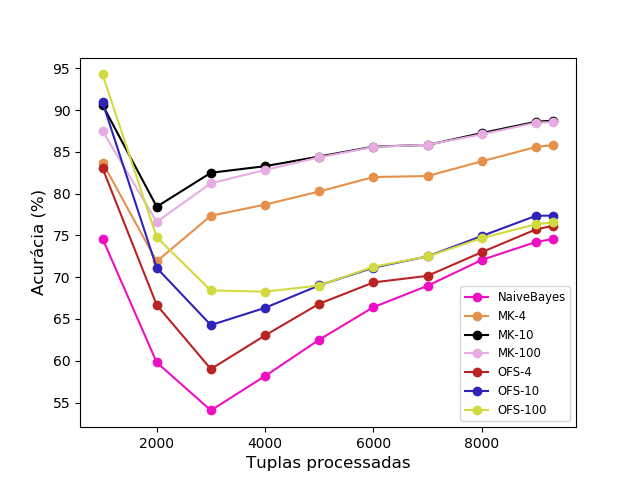
\includegraphics[width=\textwidth]{acc_spam_data.png}
\caption{Acurácia sequencial} \label{fig:spam_data_1a}
\end{subfigure}
%\hspace*{\fill} % separation between the subfigures
\hfill %[Andre] Comentei a linha anterior
\begin{subfigure}[b]{0.485\textwidth}
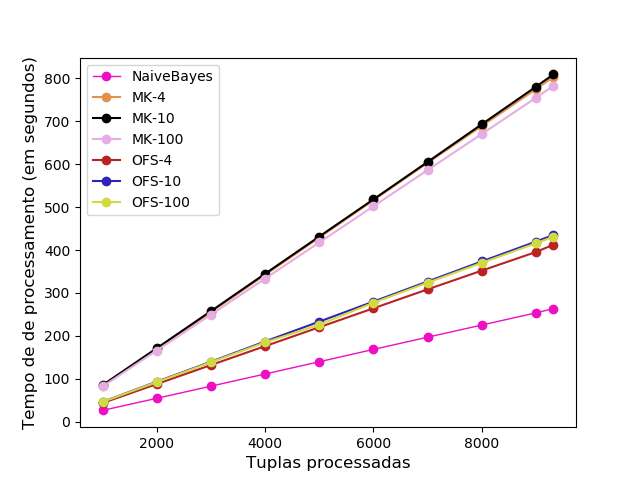
\includegraphics[width=\textwidth]{time_spam_data.png}
\caption{Tempo de resposta} \label{fig:spam_data_1b}
\end{subfigure}
%\hspace*{\fill} % separation between the subfigures
%[Andre] Comentei a linha anterior
\begin{subfigure}[b]{0.5\textwidth}
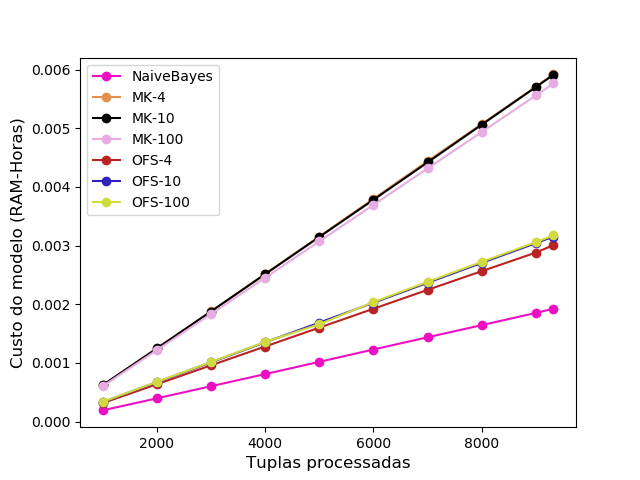
\includegraphics[width=\textwidth]{ram_spam_data.png}
\caption{Uso de memória} \label{fig:spam_data_1c}
\end{subfigure}
\caption[Gráficos de métricas no conjunto de dados \textit{spam\_data}]{Gráficos de métricas no conjunto de dados \textit{spam\_data}.} \label{fig:spam_data}
\end{figure}



\begin{figure}[!htb]
\centering
\begin{subfigure}{0.485\textwidth}
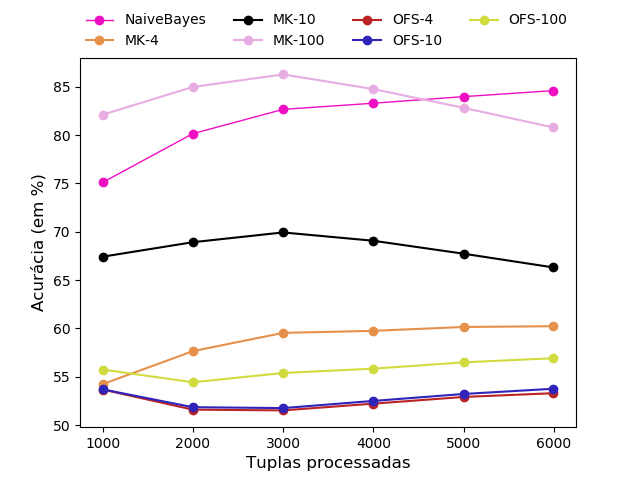
\includegraphics[width=\linewidth]{acc_mailing_list.png}
\caption{Acurácia sequencial} \label{fig:mailing_1a}
\end{subfigure}
%\hspace*{\fill} % separation between the subfigures
\hfill
\begin{subfigure}{0.48\textwidth}
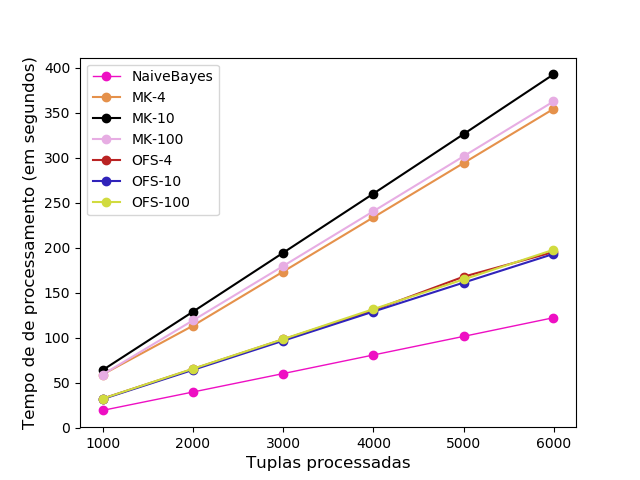
\includegraphics[width=\linewidth]{time_mailing_list.png}
\caption{Tempo de resposta} \label{fig:mailing_1b}
\end{subfigure}
%\hspace*{\fill} % separation between the subfigures
\begin{subfigure}{0.5\textwidth}
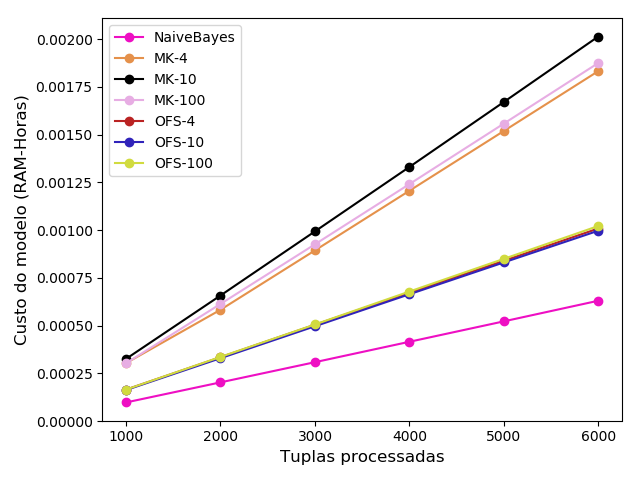
\includegraphics[width=\linewidth]{ram_mailing_list.png}
\caption{Uso de memória} \label{mailing_fig:1c}
\end{subfigure}
\caption[Gráficos de métricas no conjunto de dados \textit{mailing\_list}]{Gráficos de métricas no conjunto de dados \textit{mailing\_list}.} \label{fig:mailing_list}
\end{figure}



\begin{figure}[!htb]
\centering
\begin{subfigure}[t]{0.485\textwidth}
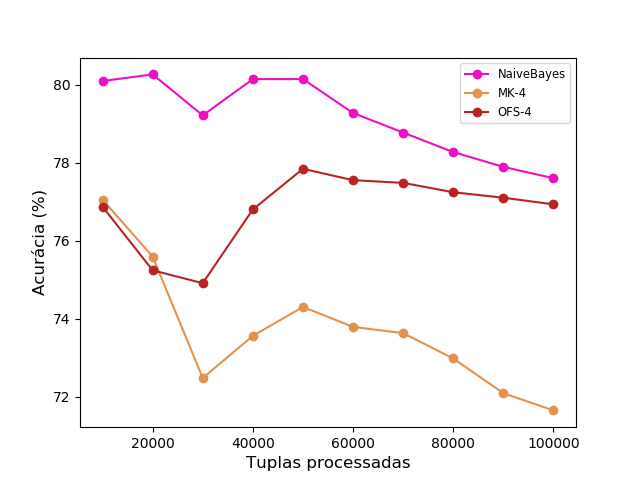
\includegraphics[width=\linewidth]{acc_incremental_drift.png}
\caption{Acurácia sequencial} \label{fig:incremental_1a}
\end{subfigure}
%\hspace*{\fill} % separation between the subfigures
\hfill
\begin{minipage}{\textwidth} 
%[Andre] Adicionei o \begin{minipage} para ajusta o restante das figuras em 4x4
% Note o \end{minipage} no final.
\begin{subfigure}[t]{0.485\textwidth}
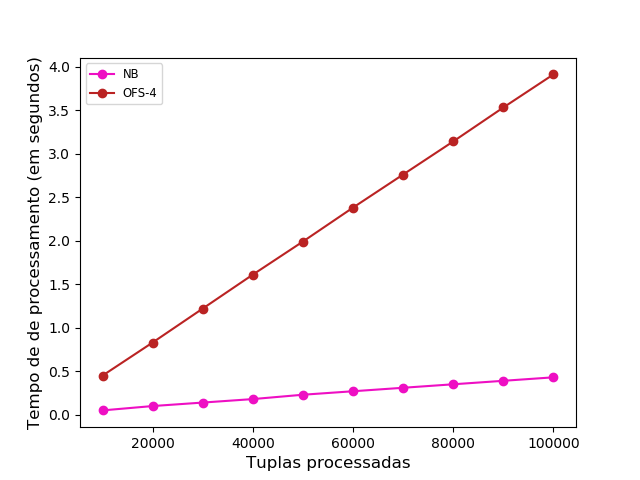
\includegraphics[width=\linewidth]{time_incremental_drift.png}
\caption{Tempo de resposta com Naïve Bayes e OFS-4} \label{fig:incremental_1b}
\end{subfigure}
%\hspace*{\fill} % separation between the subfigures
\hfill
\begin{subfigure}[t]{0.485\textwidth}
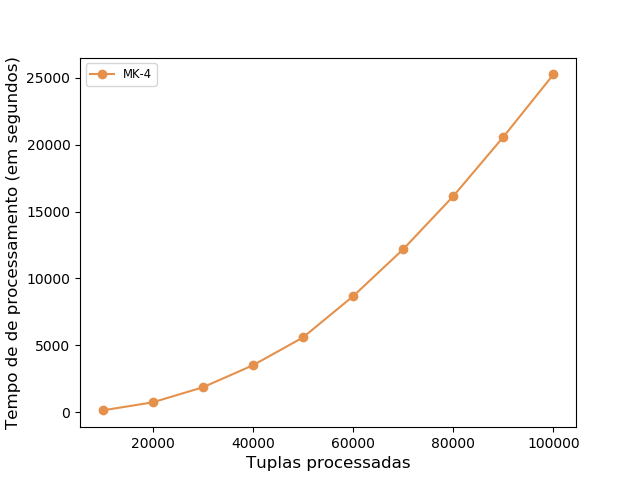
\includegraphics[width=\linewidth]{time_incremental_drift_mk4.png}
\caption{Tempo de resposta para MK-4} \label{fig:incremental_1c}
\end{subfigure}
\hfill
\begin{subfigure}[t]{0.485\textwidth}
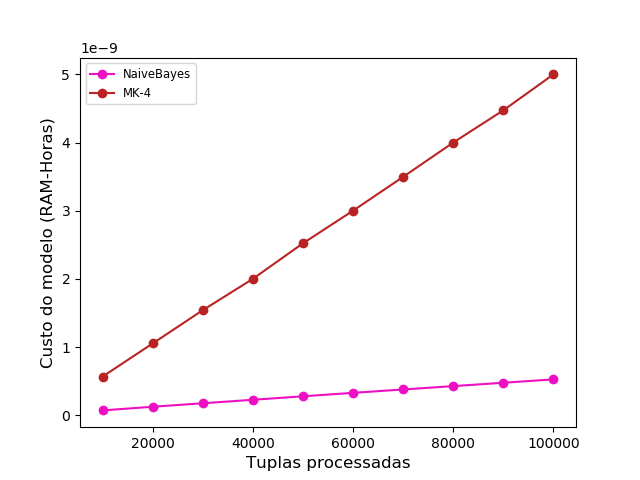
\includegraphics[width=\linewidth]{ram_incremental_drift.png}
\caption{Uso de memória com Naïve Bayes e OFS-4} \label{fig:incremental_1d}
\end{subfigure}
%\hspace*{\fill} % separation between the subfigures
\hfill
\begin{subfigure}[t]{0.485\textwidth}
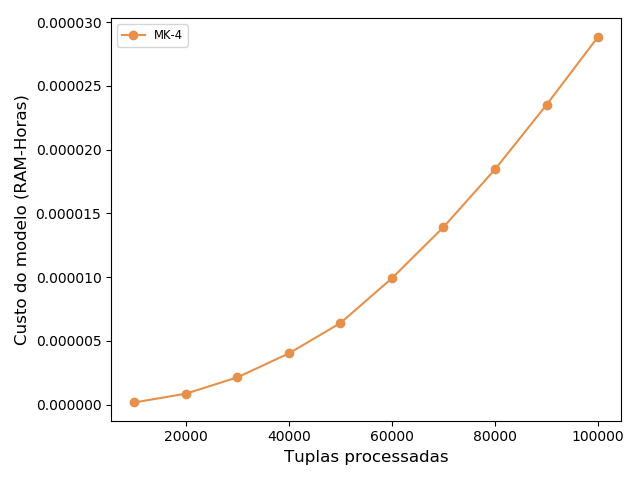
\includegraphics[width=\linewidth]{ram_incremental_drift_mk4.png}
\caption{Uso de memória para MK-4} \label{fig:incremental_1e}
\end{subfigure}
\end{minipage}

\caption[Gráficos de métricas no conjunto de dados  \textit{incremental\_drift}]{Gráficos de métricas no conjunto de dados  \textit{incremental\_drift}. Os gráficos de tempo de resposta e uso de memória precisaram ser separados para o método MK-4, devido aos altos valores.} \label{fig:incremental_drift}
\end{figure}



\begin{figure}[!htb]
\centering
\begin{subfigure}{0.485\textwidth}
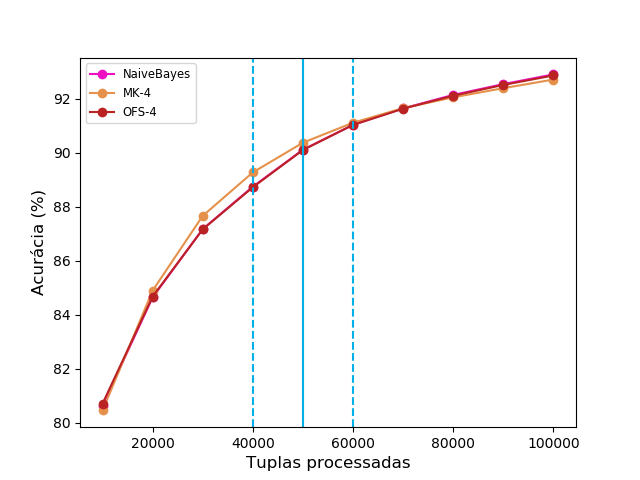
\includegraphics[width=\linewidth]{acc_gradual_drift.png}
\caption{Acurácia sequencial} \label{fig:gradual_1a}
\end{subfigure}
%\hspace*{\fill} % separation between the subfigures
\hfill
\begin{minipage}[b]{\textwidth} 
\begin{subfigure}[t]{0.485\textwidth}
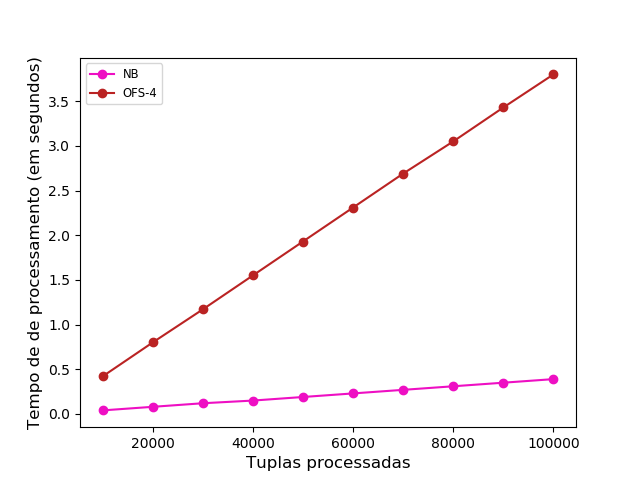
\includegraphics[width=\linewidth]{time_gradual_drift.png}
\caption{Tempo de resposta com Naïve Bayes e OFS-4} \label{fig:gradual_1b}
\end{subfigure}
%\hspace*{\fill} % separation between the subfigures
\hfill
\begin{subfigure}[t]{0.485\textwidth}
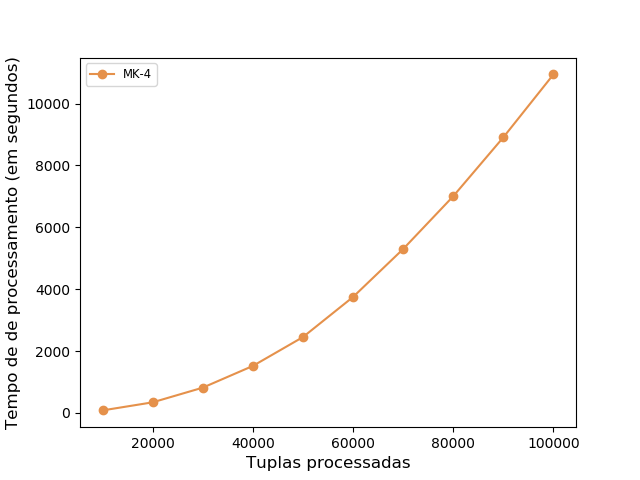
\includegraphics[width=\linewidth]{time_gradual_drift_mk4.png}
\caption{Tempo de resposta para MK-4} \label{fig:gradual_1c}
\end{subfigure}
\hfill
\begin{subfigure}[t]{0.485\textwidth}
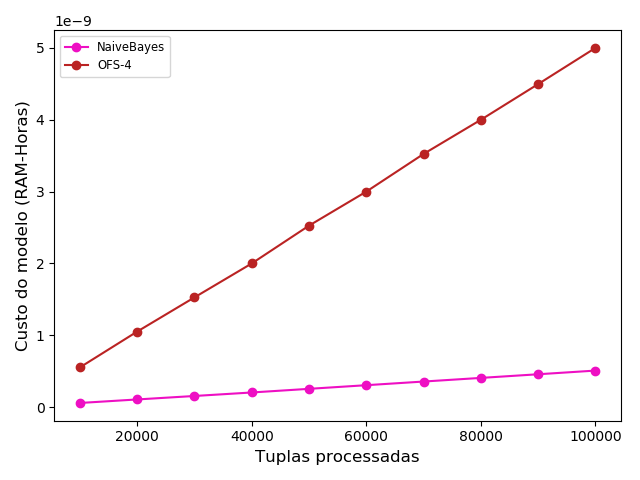
\includegraphics[width=\linewidth]{ram_gradual_drift.png}
\caption{Uso de memória com Naïve Bayes e OFS-4} \label{fig:gradual_1d}
\end{subfigure}
%\hspace*{\fill} % separation between the subfigures
\hfill
\begin{subfigure}[t]{0.485\textwidth}
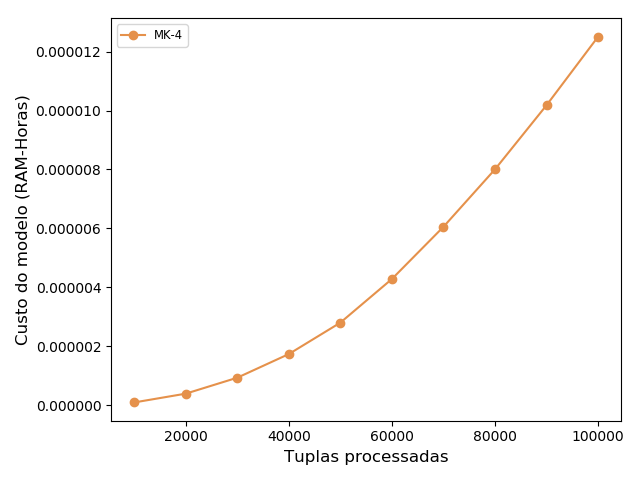
\includegraphics[width=\linewidth]{ram_gradual_drift_mk4.png}
\caption{Uso de memória para MK-4} \label{fig:gradual_1e}
\end{subfigure}
\end{minipage}

\caption[Gráficos de métricas no conjunto de dados \textit{gradual\_drift}]{Gráficos de métricas no conjunto de dados \textit{gradual\_drift}. As linhas pontilhadas e a reta em azul no gráfico de acurácia sequencial, representam, respectivamente, a janela de início/fim do \textit{drift} e o ponto exato de mudança. %Os gráficos de tempo de CPU e uso de memória precisaram ser separados para o método MK-4, devido aos altos valores.
} \label{fig:gradual_drift}
\end{figure}



\begin{figure}[!htb]
\centering
\begin{subfigure}{0.5\textwidth}
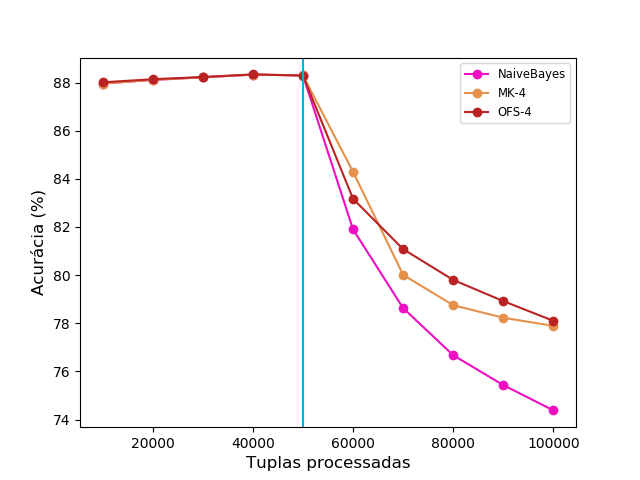
\includegraphics[width=\linewidth]{acc_sudden_drift.png}
\caption{Acurácia sequencial} \label{fig:sudden_1a}
\end{subfigure}
%\hspace*{\fill} % separation between the subfigures
\hfill
\begin{minipage}[b]{\textwidth} 
\begin{subfigure}[t]{0.485\textwidth}
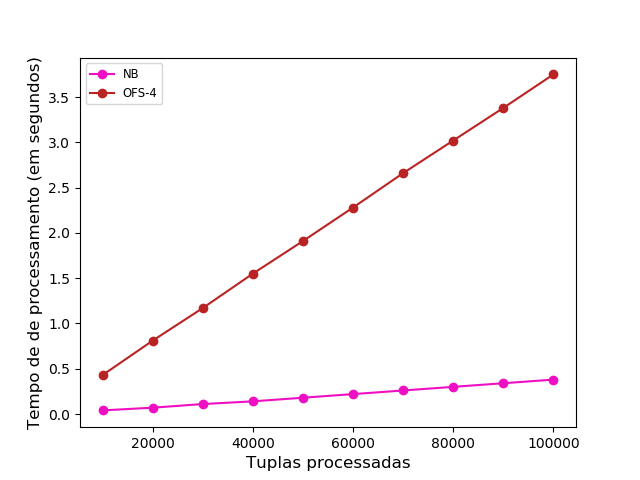
\includegraphics[width=\linewidth]{time_sudden_drift.png}
\caption{Tempo de resposta com Naïve Bayes e OFS-4} \label{fig:sudden_1b}
\end{subfigure}
%\hspace*{\fill} % separation between the subfigures
\hfill
\begin{subfigure}[t]{0.485\textwidth}
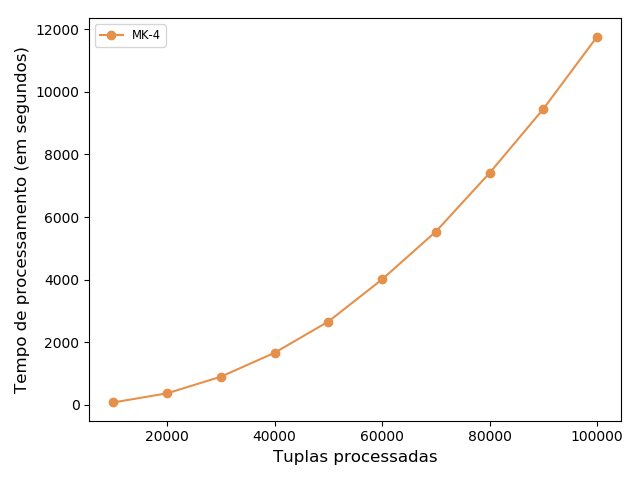
\includegraphics[width=\linewidth]{time_sudden_drift_mk4.png}
\caption{Tempo de resposta para MK-4} \label{fig:sudden_1c}
\end{subfigure}
\hfill
\begin{subfigure}[t]{0.485\textwidth}
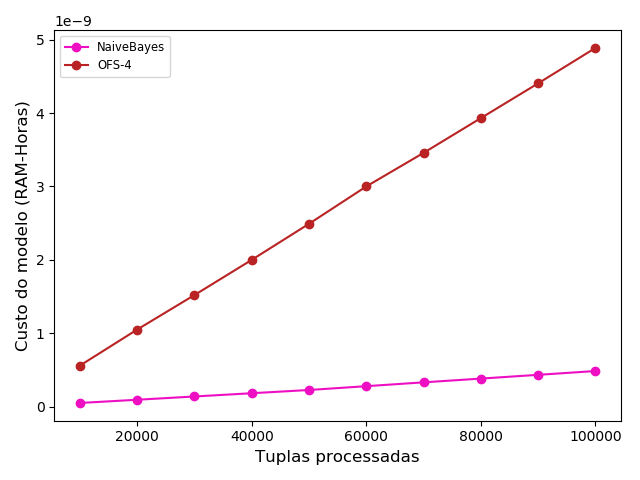
\includegraphics[width=\linewidth]{ram_sudden_drift.png}
\caption{Uso de memória com Naïve Bayes e OFS-4} \label{fig:sudden_1d}
\end{subfigure}
%\hspace*{\fill} % separation between the subfigures
\hfill
\begin{subfigure}[t]{0.485\textwidth}
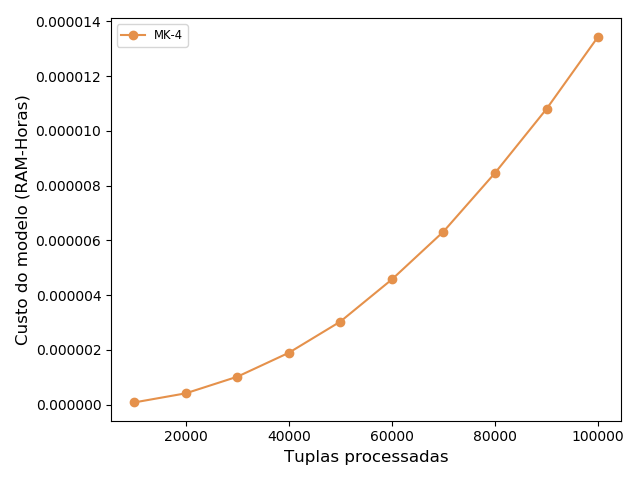
\includegraphics[width=\linewidth]{ram_sudden_drift_mk4.png}
\caption{Uso de memória para MK-4} \label{fig:sudden_1e}
\end{subfigure}
\end{minipage}

\caption[Gráficos de métricas no conjunto de dados \textit{sudden\_drift}]{Gráficos de métricas no conjunto de dados \textit{sudden\_drift}. A linha reta em azul no gráfico de acurácia sequencial representa o ponto exato de mudança. %Os gráficos de tempo de resposta e uso de memória precisaram ser separados para o método MK-4, devido aos altos valores.
} \label{fig:sudden_drift}
\end{figure}



\begin{figure}[!htb]
\centering
\begin{subfigure}{0.5\textwidth}
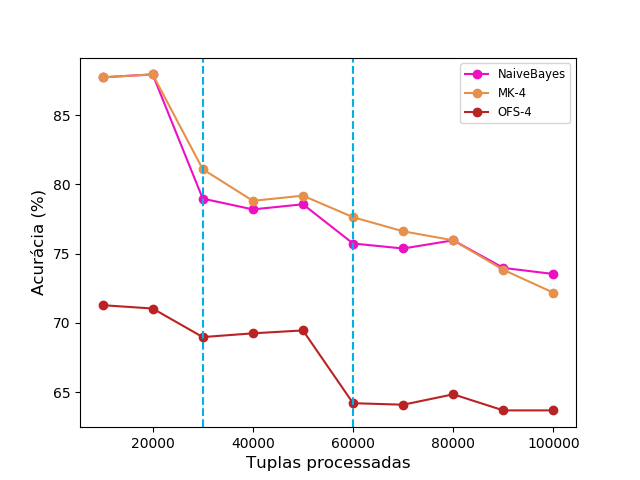
\includegraphics[width=\linewidth]{acc_recurrent_drift.png}
\caption{Acurácia sequencial} \label{fig:recurrent_1a}
\end{subfigure}
%\hspace*{\fill} % separation between the subfigures
\hfill
\begin{minipage}[b]{\textwidth} 
\begin{subfigure}[t]{0.485\textwidth}
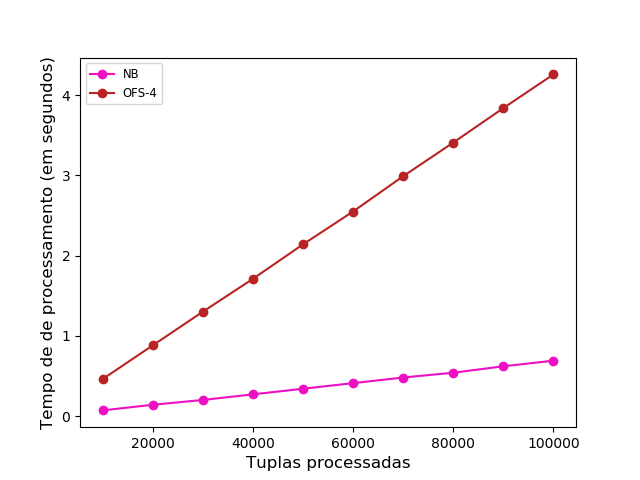
\includegraphics[width=\linewidth]{time_recurrent_drift.png}
\caption{Tempo de resposta com Naïve Bayes e OFS-4} \label{fig:recurrent_1b}
\end{subfigure}
%\hspace*{\fill} % separation between the subfigures
\hfil
\begin{subfigure}[t]{0.485\textwidth}
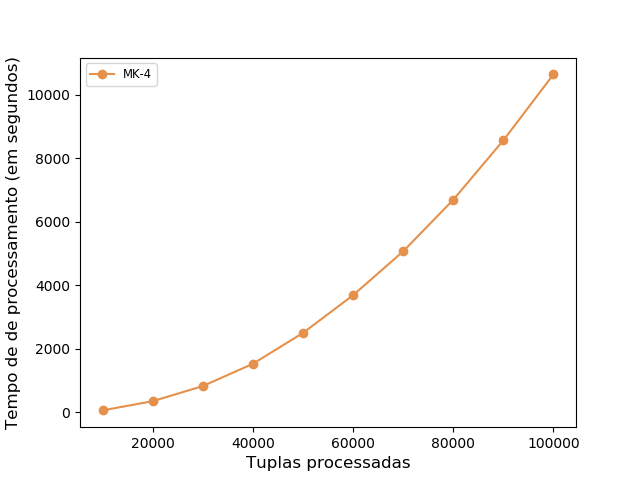
\includegraphics[width=\linewidth]{time_recurrent_drift_mk4.png}
\caption{Tempo de resposta para MK-4} \label{fig:recurrent_1c}
\end{subfigure}
\hfill
\begin{subfigure}[t]{0.485\textwidth}
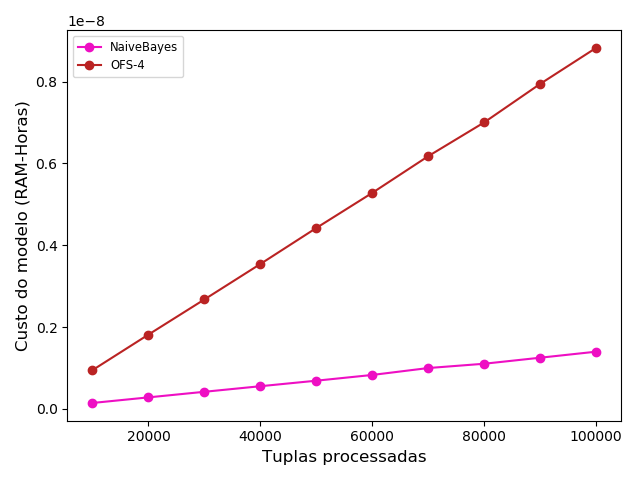
\includegraphics[width=\linewidth]{ram_recurrent_drift.png}
\caption{Uso de memória com Naïve Bayes e OFS-4} \label{fig:recurrent_1d}
\end{subfigure}
%\hspace*{\fill} % separation between the subfigures
\hfill
\begin{subfigure}[t]{0.485\textwidth}
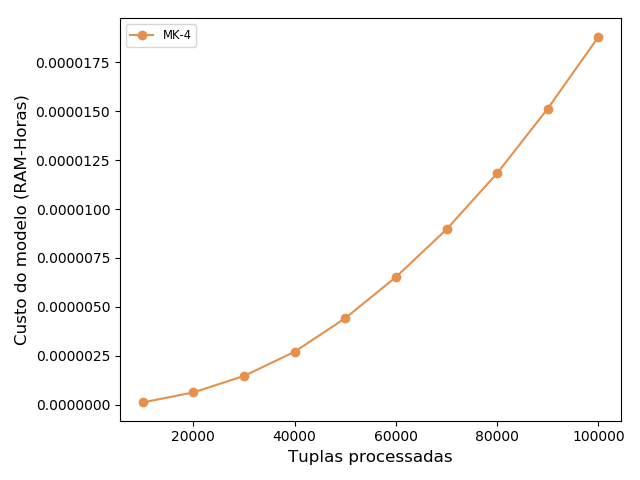
\includegraphics[width=\linewidth]{ram_recurrent_drift_mk4.png}
\caption{Uso de memória para MK-4} \label{fig:recurrent_1e}
\end{subfigure}
\end{minipage}

\caption[Gráficos de métricas no conjunto de dados \textit{recurrent\_drift}]{Gráficos de métricas no conjunto de dados \textit{recurrent\_drift}. As linhas pontilhadas no gráfico de acurácia sequencial representam respectivamente o início/fim da mudança. %Os gráficos de tempo de resposta e uso de memória precisaram ser separados para o método MK-4, devido aos altos valores.
} \label{fig:recurrent_drift}
\end{figure}

%[Andre] justei essa seção à anterior.
%\section{Discussões}\label{sec:res_discussoes}

\begin{figure}[!htb]
\centering
\begin{subfigure}[b]{0.485\textwidth}
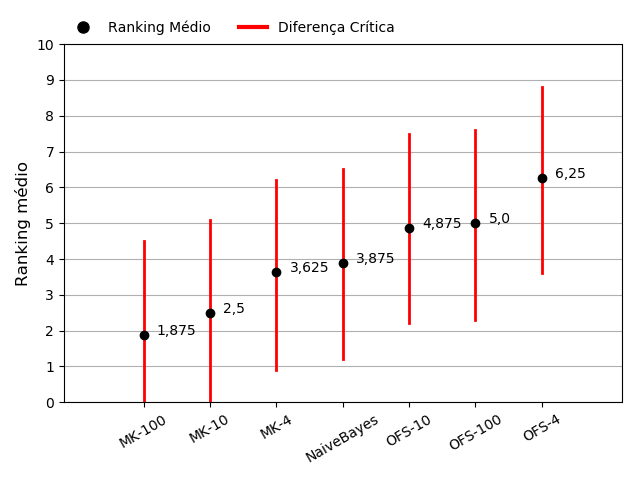
\includegraphics[width=\textwidth]{bonferroni_real.png}
\caption{Conjuntos de dados reais} \label{fig:bonferroni_1a}
\end{subfigure}
%\hspace*{\fill} % separation between the subfigures
\hfill %[Andre] Comentei a linha anterior
\begin{subfigure}[b]{0.485\textwidth}
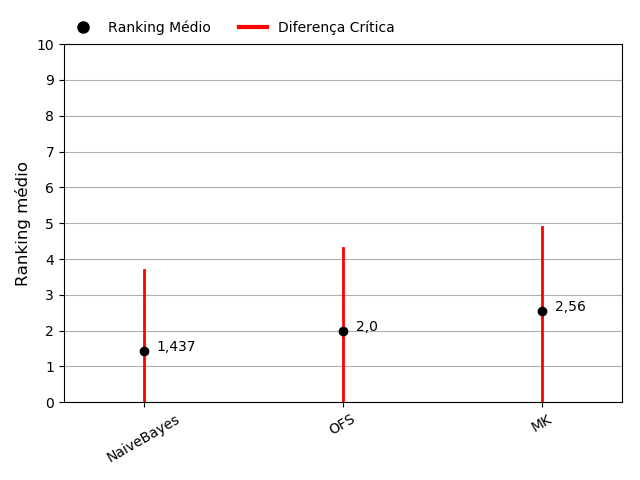
\includegraphics[width=\textwidth]{bonferroni_artificial.png}
\caption{Conjuntos de dados artificiais} \label{fig:bonferroni_1b}
\end{subfigure}
\caption{Gráficos de diferença crítica com o teste \textit{post-hoc} de Bonferroni-Dunn} \label{fig:bonferroni}
\end{figure}



Os resultados dos experimentos apontam  que o algoritmo MK apresentou os piores resultados em termos de tempo de resposta e quantidade de memória em todas as situações. Nos conjuntos de dados artificiais e com a janela de processamento tupla a tupla ($winSize=1$), chegou a consumir um tempo 500.000 vezes maior que os demais (7 horas contra aproximadamente 5 segundos para NB e OFS). Nas situações onde a janela de processamento foi maior,  o desempenho do MK foi relativamente superior aos obtidos pelo mesmo algoritmo. 

No conjunto \textit{incremental\_drift}, onde apresentou o pior resultado de todos em tupla a tupla, com $winSize=10$, o tempo de resposta foi reduzido em 700\%, atingindo cerca de 1 hora de processamento. Com $winSize=100$, passou para 5 minutos e, por fim, com $winSize=1000$, executou em 25 segundos. Neste último, a acurácia foi superior às outras janelas. Entretanto, ainda bem abaixo que a obtida com NB. O consumo de memória, consequentemente, também foi reduzido nessas proporções.

Quanto ao OFS, o mesmo possui velocidades competitivas ao NB. No pior cenário, com $winSize=1$ no conjunto de dados \textit{incremental\_drift}, analisou e classificou todas as tuplas em 5 segundos. Com $winSize=10,100 \text{ e } 1000$, precisou de, respectivamente, 
1,5 segundos, 0,9 segundos e 0,5 segundos.Neste último, ficou apenas 0,07 segundos atrás 
do algoritmo NB. Quanto ao consumo de memória, no pior dos cenários, o algoritmo OFS
precisou de $5\times10^{-9}$ RAM-horas e no melhor $5.2\times10^{-10}$ RAM-horas. Esse último valor é exatamente o mesmo obtido utilizando apenas o algoritmo NB.

Por fim, para validar os resultados de acurácia obtidos nos experimentos, foi utilizado o teste de Friedman, conforme indicado no Capítulo~\ref{chp:referencial}. Para um intervalo de confiança de $\alpha = 0,05$, o teste de Friedman indicou que a hipótese nula foi rejeitada. Diante disso, foi verificado se os resultados obtidos pelo NB foram significativamente superiores aos de MK e OFS utilizando o teste \textit{post-hoc} de Bonferroni-Dunn. A Figura~\ref{fig:bonferroni}, na página \pageref{fig:bonferroni}, apresenta os resultados para ambos os conjuntos de dados reais e artificiais, considerando todas as janelas de processamento.

Para os conjuntos reais e artificiais, em um intervalo de confiança de $\alpha=0,05$, a diferença crítica foi $2,638$ e $2,343$, respectivamente. Analisando os resultados, há evidências de que, embora o NB obtenha acurácias finais superiores na maioria dos cenários (4 de 6), essa superioridade não é significativa, pois considerando bases de dados reais e artificiais seus resultados são estatisticamente equivalentes aos de MK e OFS. Esses resultados estão abaixo da diferença crítica em todos os cenários avaliados. 

\citeonline{Katakis2005} apresentam em seu artigo os resultados da acurácia de seu método utilizando o conjunto de dados \textit{spam\_data}. Esses resultados são similares aos obtidos nos experimentos aqui apresentados. Entretanto, os autores não avaliam nenhuma outra métrica. Desse modo, os experimentos deste trabalho demonstram que, embora a acurácia final seja de fato razoável, o consumo de memória e tempo de resposta elevados inviabilizam a utilização deste método. 

Entretanto, analisando as acurácias sequenciais desse algoritmo, o mesmo apresenta a melhor adaptabilidade a mudanças de conceitos graduais e súbitas quando a dimensionalidade dos fluxos é alta e justifica a utilização de seleção de atributos, e nos casos de mudanças recorrentes, mesmo em baixa dimensionalidade. Esse fato demonstra que há potencial na utilização deste método em cenários de mudanças de conceito, em especial em cenários de alta dimensionalidade, caso o tempo de resposta e o consumo de memória RAM sejam reduzidos.

Uma possível solução para esse cenário é a utilização da Computação de Alto Desempenho para a utilização de bibliotecas que permitam que os trechos de código mais custosos computacionalmente sejam paralelizados. Outra alternativa é a utilização de Unidades de Processamento Gráfico (\textit{Graphics Processing Units -- GPU}) para realização do cálculo de avaliação dos atributos. Desta forma, o processador ficaria responsável apenas pela classificação dos dados, o que diminuiria a carga de trabalho e concorrência, reduzindo o tempo necessário para avaliação dos atributos e consequentemente da classificação final.

Em seu artigo, \citeonline{Wang2014} apresentam os resultados de uma avaliação sistemática do desempenho do OFS em diferentes situações, em especial com conjuntos de dados em larga escala. Nesses cenários, o algoritmo OFS demonstra uma alta capacidade para lidar com grandes volumes de dados, tanto no número de tuplas quanto na quantidade de atributos, em situações onde não há variação probabilística dos dados. 

Contudo, os experimentos realizados neste trabalho apontam que o algoritmo OFS é sensível à mudanças de conceitos, apresentando acurácia inferior ao algoritmo NB em cinco dos seis cenários avaliados. Além disso, também obteve uma acurácia inferior ao MK em conjuntos de dados com alta dimensionalidade, o que pode torná-lo inviável nessas situações. Avaliando a acurácia sequencial, o OFS mostrou a maior adaptabilidade à mudanças súbitas quando a dimensão dos dados é baixa. 

Desse modo, as evidências apontam que, no geral,  a utilização de um método de classificação supervisionada sem a seleção de atributos apresenta resultados superiores quando comparados a utilização do Método de Katakis com Ganho de Informação e o algoritmo \textit{OnlineFeatureSelection} em fluxos de dados com mudanças de conceito. Entretanto, por apresentar uma maior adaptabilidade às mudanças de conceito no quesito capacidade preditiva em três dos seis cenários, o Método de Katakis com Ganho de Informação possui um potencial de utilização caso seus problemas de desempenho sejam solucionados.


\section{Considerações finais deste capítulo}\label{sec:res_consideracoes} 

Este capítulo apresentou os resultados dos experimentos realizados com os algoritmos MK e OFS. O algoritmo MK apresentou os piores tempos de resposta e consumo de memória, mas acurácias aproximadas da classificação sem seleção de atributos (apenas com NB), superando-o em uma situação e superior ao OFS em quatro dos seis cenários. 

Já o algoritmo OFS demonstrou tempos de resposta e consumo de memória relativamente próximos aos obtidos com o algoritmo NB. Em termos de acurácia, o algoritmo OFS mostrou maior adaptabilidade às mudanças súbitas em fluxos com uma baixa dimensionalidade, superando os demais algoritmos considerados nesse cenário. Contudo, esse algoritmo obteve resultados inferiores em conjuntos com alta dimensionalidade.

A hipótese nula de semelhança dos algoritmos foi rejeitada com o teste de Friedman, e o teste \textit{post-hoc} de Bonferroni-Dunn apresentou evidências de equivalência estatística das acurácias de NB em comparação com MK e OFS em todos os cenários. 

% O comando a seguir inclui o arquivo conclusoes.tex
% que contém o capítulo de conclusoes. 
% Detalhe: não precisa incluir a extensão .tex
\chapter{Conclusões Parciais}\label{chp:conclusoes}

Algoritmos de seleção de atributos podem ser uma ferramenta útil para reduzir, em tempo real, a dimensão dos fluxos de dados. Desse modo, a classificação desses fluxos por parte dos sistemas de processamento de eventos complexos pode se tornar menos custosa, mais rápida e eficiente. Todavia, para que esse potencial seja atingido, esses algoritmos devem demonstrar uma habilidade de se adaptar ao fenômeno de mudança de conceito da qual os fluxos de dados estão sujeitos.

Os resultados parciais deste trabalho apontam que os algoritmos de seleção de atributos Método de Katakis com Ganho de Informação e \textit{Online Feature Selection} demandam um maior consumo de memória e um maior tempo de resposta para classificação dos fluxos de dados, em relação à não utilização de nenhum método de seleção de atributos (usando apenas o classificador Naïve Bayes). Quanto à acurácia, o teste de Bonferroni-Dunn apresentou evidências que, embora o Naïve Bayes apresente resultados finais superiores em 4 de 6 situações, essa superioridade não é significativa, pois ficou abaixo da diferença crítica em todos os cenários.

O Método de Katakis obteve o pior tempo de resposta e consumo de memória em todos os cenários. Entretanto, apresentou acurácias competitivas com a classificação sem seleção de atributos, superando-o em conjuntos de dados reais, com alta dimensionalidade. Além disso, superou as acurácias do OFS em três dos seis cenários. Deste modo, há um potencial para utilização deste método caso seu desempenho computacional seja melhorado. Algumas possíveis soluções envolvem o uso de bibliotecas para Computação de Alto Desempenho que paralelizem o código ou o uso de unidades de processamento gráfico para realização da avaliação dos atributos, diminuindo a carga de trabalho do processador.

O algoritmo OFS, em contrapartida, apresentou consumo de memória e tempo de resposta relativamente próximos aos obtidos sem a utilização da seleção de atributos. Além disso, demonstrou uma maior adaptabilidade quando comparado ao MK em cenários de mudanças súbitas, quando a dimensão dos dados é pequena. Contudo, sua acurácia em conjuntos de dados com alta dimensionalidade foi inferior ao MK, o que indica que embora veloz e com baixo custo computacional, seu uso com grandes quantidades de atributos pode ser inviável.

Para a continuação dessa pesquisa, serão implementados e testados os quatro algoritmos restantes. Após o final dessa avaliação, pretende-se implementar algumas das soluções propostas a fim de verificar se o desempenho dos algoritmos pode ser melhorado. 


\chapter{Cronograma}\label{chp:cronograma}

A Tabela \ref{tab_cronograma} apresenta as atividades realizadas e previstas para este trabalho. A tabela está dividida em bimestres, começando em julho de 2017, quando ingressei oficialmente no Programa de Pós-graduação da Faculdade de Tecnologia da UNICAMP.

\begin{table}[!htp]
\centering
\caption{Cronograma de execução das atividades}
\label{tab_cronograma}
\begin{threeparttable}[b]
\begin{tabular}{|p{3.1cm}|c|c|c|c|c|c|c|c|c|c|c|c|c|}
\hline
                                              & \multicolumn{3}{c|}{2017}                                                                                                                           & \multicolumn{6}{c|}{2018}                                                                                                                                                                                                                                                                                 & \multicolumn{4}{c|}{2019}                                                                                                                                                                             \\ \hline
\multicolumn{1}{|c|}{\textbf{Atividade / Bim.}}               & \begin{tabular}[c]{@{}c@{}}4º\end{tabular} & \begin{tabular}[c]{@{}c@{}}5º\end{tabular} & \begin{tabular}[c]{@{}c@{}}6º\end{tabular} & \begin{tabular}[c]{@{}c@{}}1º\end{tabular} & \begin{tabular}[c]{@{}c@{}}2º\end{tabular} & \begin{tabular}[c]{@{}c@{}}3º\end{tabular} & \begin{tabular}[c]{@{}c@{}}4º\end{tabular} & \begin{tabular}[c]{@{}c@{}}5º\end{tabular} & \begin{tabular}[c]{@{}c@{}}6º\end{tabular} & \begin{tabular}[c]{@{}c@{}}1º\end{tabular} & \begin{tabular}[c]{@{}c@{}}2º\end{tabular} & \begin{tabular}[c]{@{}c@{}}3º\end{tabular} & \begin{tabular}[c]{@{}c@{}}4º\end{tabular} \\ \hline
Integralização curricular                     & O                                               & O                                               & O                                               & O                                               & O                                               & O                                               &                                               &                                                 &                                                 &                                                 &                                                 &                                                 &                                                 \\ \hline
Revisão bibliográfica                         & O                                               & O                                               & O                                               & O                                               & O                                               & O                                               &                                                &                                                &                                               &                                                 &                                               &                                               &                                                 \\ \hline
Introdução a Data Stream e Concept Drift      & O                                               & O                                               &                                                 &                                                 &                                                 &                                                 &                                                 &                                                 &                                                 &                                                 &                                                 &                                                 &                                                 \\ \hline
Definição de técnicas a serem implementadas   &                                                 & O                                               & O                                               & O                                                & O                                               &                                                 &                                                 &                                                 &                                                 &                                                 &                                                 &                                                 &                                                 \\ \hline
Escrita da Qualificação                       &                                                 &                                                 &                                                & O                                               & O                                               & O                                               &                                                 &                                                 &                                                 &                                                 &                                                 &                                                 &                                                 \\ \hline
Definição e caracterização das bases de dados &                                                 &                                                 &                                                 & O                                               & O                                               & O                                               & X                                                &                                                 &                                                 &                                                 &                                                 &                                                 &                                                 \\ \hline
Exame de Qualificação                         &                                                 &                                                 &                                                 &                                                 &                                                 &                                                 & X                                               &                                                 &                                                 &                                                 &                                                 &                                                 &                                                 \\ \hline
Implementação dos algoritmos propostos        &                                                 &                                                 &                                                 &                                                 &                                                 & O                                               & X                                               & X                                               & X                                               & X                                               &                                                 &                                                 &                                                 \\ \hline
Obtenção de resultados                        &                                                 &                                                 &                                                 &                                                 &                                                 & O                                               & X                                                & X                                               & X                                               & X                                               & X                                                &                                                 &                                                 \\ \hline
Elaboração de artigos                         &                                                 &                                                 &                                                 &                                                 &                                                 &                                                 &                                                 &                                                 & X                                               & X                                               & X                                               & X                                               &                                                 \\ \hline
Escrita da dissertação                        &                                                 &                                                 &                                                &                                                 &                                                &                                                 &                                                &                                                 & X                                               & X                                               & X                                               & X                                               &                                                 \\ \hline
Defesa                                        &                                                 &                                                 &                                                 &                                                 &                                                 &                                                 &                                                 &                                                 &                                                 &                                                 &                                                 &                                                 & X                                               \\ \hline
\end{tabular}
\begin{tablenotes}
\item[1]O -- Concluído; X -- Pendente.
\end{tablenotes}
\end{threeparttable}
\end{table}

A integralização curricular foi composta por disciplinas cursadas na Faculdade de Tecnologia da UNICAMP, inicialmente como aluno especial, e a partir de Agosto de 2017, como aluno regular.

Após o ingresso como regular, foi solicitado o aproveitamento de estudos das disciplinas e com a realização das disciplinas obrigatórias restantes, o total de 24 créditos necessários foi atingido como se segue:

\begin{itemize}
\item Obrigatórias:
\begin{itemize}
\item FT055 -- 4 créditos -- Inovação e Transferência de Tecnologias (2017);
\item FT054 -- 4 créditos -- Pesquisa Científica: Concepção, Desenvolvimento e Publicação (2018);
\end{itemize}
\item Eletivas I:
\begin{itemize}
\item FT060 -- 4 créditos -- Matemática Discreta (2017);
\end{itemize}
\item Eletivas II:
\begin{itemize}
\item FT043 -- 4 créditos -- Tópicos em Tecnologia para Informação I (Mineração de Dados) (2017);
\item FT077 -- 4 créditos -- Processamento de Alto Desempenho (2017);
\item FT057 -- 4 créditos -- Ferramentas Estatísticas e Computacionais para Ciência e Tecnologia (2017);
\end{itemize}
\end{itemize}

Sendo assim, até a realização do exame de qualificação, todas as disciplinas necessárias para o cumprimento da carga horária exigida para o programa foram cursadas. Portanto, o tempo restante para conclusão do projeto de mestrado será dedicado para realização dos experimentos restantes, desenvolvimento dos testes, coleta dos resultados e escrita de artigos e da dissertação.



% Os comandos para as referências bibliográficas estão a seguir
% Estilo de bibliografia. Nesse caso é o estilo alfabético.
\bibliographystyle{abntex2-alf}
% As referências bibliográficas estão no arquivo 
% bibliografia.bib . Nesse caso, coloque o arquivo sem a
% extensão .bib.
\bibliography{bibliografia}

% Os anexos, se houver, vêm depois das referências:
\appendix

\chapter{Método PRISMA para revisão bibliográfica}

Este apêndice descreve a metodologia de revisão sistemática utilizada para pesquisar as referências bibliográficas utilizadas neste trabalho. O método utiliza 9 etapas, baseadas no \textit{framework} PRISMA \cite{Moher2010}. Estas etapas são: 1) definição do tópico de pesquisa, 2) definição dos conceitos envolvidos, 3) seleção das fontes bibliográficas, 4) definição dos termos de busca, 5) definição da estratégia de pesquisa, 6) critérios de seleção e 7) construção do diagrama de fluxos. Cada um dos passos citados será mostrado como se segue:

\section{Definição do tópico de pesquisa}\label{sec:prisma_topico} 

Esta etapa especificou o tópico que orientou a definição dos conceitos envolvidos nesta pesquisa. O tópico de pesquisa escolhido foi: ``Redução de dados em fluxos de dados com mudança de conceito''.

\section{Definição dos conceitos envolvidos }\label{sec:prisma_conceitos} 

Com base na pesquisa de definição de tópicos, foram identificados três conceitos envolvidos: 1) \textit{Data Streams}; 2) \textit{Concept Drift}; 3) \textit{Data Reduction}. Esses conceitos serão descritos a seguir:

\begin{itemize}
\item \textit{Data Streams}: é uma sequência ordenada e potencialmente infinita de instâncias, transmitidas em alto volume e alta velocidade, o que impede seu completo armazenamento em memória. Diante desses fatores, tais instâncias precisam ser analisadas em tempo real.
\item \textit{Concept Drift}: É uma mudança inesperada na relação de um conjunto de variáveis $X$ a uma saída $y$ durante um intervalo de tempo. A definição formal é dada por: $ \exists X : p_t0 (X,y) \neq p_t1 (X,y) $ e.g. dados de sensores usados para captação de abalos sísmicos podem variar inesperadamente em caso de um princípio de terremoto.
\item \textit{Data Reduction}: técnicas de pré-processamento que visam reduzir um determinado conjunto de dados à uma representação menor em volume, porém mantendo a qualidade estatística das informações. Essas técnicas podem ser usadas tanto para reduzir as instâncias quanto os atributos do conjunto de dados.
\end{itemize}

\section{Seleção das fontes bibliográficas }\label{sec:prisma_fontes} 

As pesquisas foram realizadas nas bases IEEE Xplore, Science Direct, ACM Digital Library e Web of Science. Pesquisas manuais em bibliotecas, bem como artigos indicados pelo orientador ou outros especialistas foram realizadas em paralelo. Os artigos, livros ou dissertações/teses obtidas por esses meios não serão descritos neste apêndice.

\section{Definição dos termos de busca}\label{sec:prisma_termos} 

Os termos de pesquisa foram especificados pela observação das palavras-chave pertinentes à este trabalho e por indicações do orientador. Assim, os termos de pesquisa utilizados foram:  1) \textit{Data Streams}; 2) \textit{Concept Drift} e 3) \textit{Data Reduction}. No IEEE Xplore, a pesquisa foi realizada com base no campo ``Full Text and Metadata''. No ScienceDirect, não foi especificado nenhum campo, para que a pesquisa abrangesse todos os textos na íntegra. Na ACM Digital Library, também não foi selecionado nenhum campo específico. Na base Web of Science, foi selecionada a aba ``Advanced Search'', utilizando a busca por tópico (\textit{topic search} -- TS). 

\section{Definição da estratégia de pesquisa}\label{sec:prisma_estrategia} 

Um exemplo de estratégia de pesquisa no ScienceDirect pode ser vista na Tabela~\ref{tab_estr_pesquisa} a seguir.

\begin{table}[!htp]
\centering
\caption{Exemplo de estratégia de pesquisa para ScienceDirect e número de \textit{hits} retornados}

\label{tab_estr_pesquisa}
\begin{tabular}{|l|}
\hline
\begin{tabular}[c]{@{}l@{}}\textbf{1. Data Streams (18,882)}\\ (``Data Streams'')\end{tabular}                                                                   \\ \hline
\begin{tabular}[c]{@{}l@{}}\textbf{2. Concept Drift (548)}\\ (``Concept Drift'')\end{tabular}                                                                    \\ \hline
\begin{tabular}[c]{@{}l@{}}\textbf{3. Data Reduction (60,451)}\\ (``Data Reduction'')\end{tabular}                                                                    \\ \hline
\begin{tabular}[c]{@{}l@{}}\textbf{4. Pesquisa Final (889)}\\ \textbf{( 1  AND 2 ) OR (1 AND 3 )}\\ (``Data Streams'' AND ``Concept Drift'') OR (``Data Streams'' AND ``Data Reduction'')\end{tabular} \\ \hline
\end{tabular}
\end{table}

Após a realização da pesquisa, um gráfico com a quantidade de publicações por ano foi gerado, como pode ser visto na Figura~\ref{fig:referencias}.

\begin{figure}[!htb]
\centering
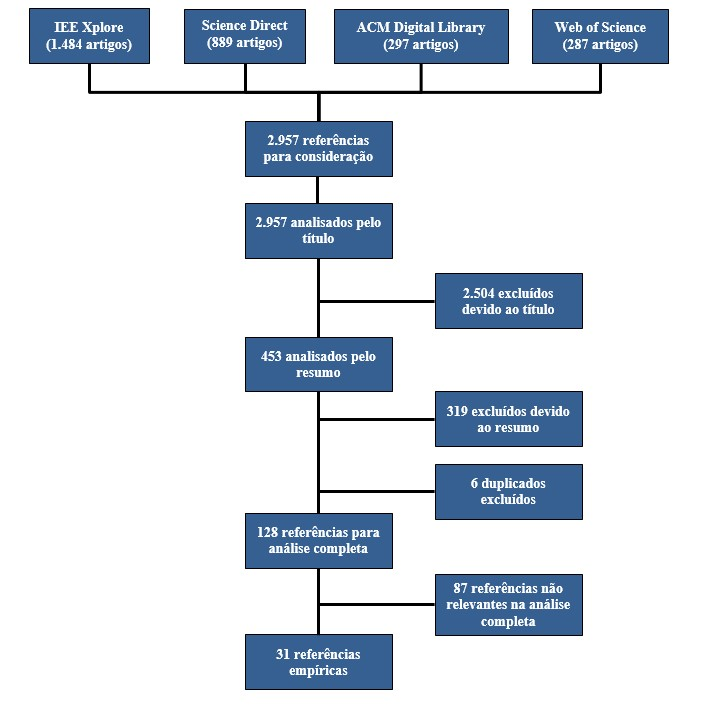
\includegraphics[scale=0.8]{referencias.jpg}
\caption{Revisão Sistemática}
\label{fig:referencias}
\end{figure}

\section{Critérios de Seleção}\label{sec:prisma_criterios} 

Após a execução da pesquisa, cada artigo foi submetido a um conjunto de critérios de elegibilidade, visando a obtenção dos artigos que fossem pertinentes a este trabalho. Todos aqueles que não se enquadraram nos critérios estabelecidos foram excluídos. Os critérios utilizados para avaliação dos artigos nas etapas de título inicial e resumo foram: o assunto é lidar com \textit{Concept Drift} e/ou \textit{Data Reduction} em \textit{Data Streams}. Sendo assim, foram definidos os seguintes critérios:
\begin{itemize}
\item É uma proposta ou implementação de algoritmo de redução de dados em\textit{Data Streams};
\item É uma proposta ou implementação para lidar com o fenômeno de \textit{Concept Drift} em \textit{Data Streams};
\item É uma pesquisa recente ou referência teórica.
\end{itemize}

Quanto a etapa de leitura completa do texto, os critérios utilizados foram:

\begin{itemize}
\item análise do método utilizado;
\item análise dos resultados;
\item análise de contribuição relevante.
\end{itemize}

Ao final, uma análise completa e detalhada de cada um dos artigos selecionados a partir dos critérios acima especificados foi realizada. Os resultados obtidos durante essa análise foram utilizados para compor a Tabela~\ref{tab_pontos-chave_artigos}, que apresenta os principais pontos de cada artigo selecionado. Os detalhes são apresentados a seguir.

\section{Diagrama de Fluxo}\label{sec:prisma_diagrama} 

As primeiras pesquisas resultaram em 2.957 referências, 31 das quais foram selecionadas por cumprirem os critérios de elegibilidade, de acordo com a Figura~\ref{fig:referencias}. As características dessas 31 referências e seus pontos chave são apresentados na Tabela~\ref{tab_pontos-chave_artigos}. 



\begin{longtable}[c]{|p{2.7cm}|p{5cm}|p{7cm}|}
\caption{Referências levantadas e seus pontos-chave}
\label{tab_pontos-chave_artigos}
\\ \hline
\textbf{Autor (ano)}            & \textbf{Título da referência}                                                                                                   & \textbf{Pontos Chave}                                                                                                                                                     
\\
\endfirsthead  

\multicolumn{3}{c}%
{{\tablename\ \thetable{} -- continuação da página anterior}} \\
\hline
\textbf{Autor (ano)}            & \textbf{Título da referência}                                                                                                   & \textbf{Pontos Chave}                                                                                                                                                     
\\
\endhead

\hline \multicolumn{3}{|r|}{{Continua na próxima página...}} \\ \hline
\endfoot

\endlastfoot

\hline
\cite{Goncalves2014}  & A comparative study on concept drift detectors & Artigo com um estudo comparativo entre detectores de concept drift, que apresenta vários tipos existentes e seus desempenhos diante de alguns critérios. Apresenta datasets importantes e previamente utilizados na área de concept drift.         
\\ \hline
\cite{Carmona-Cejudo2013} & A comparative study on feature selection and adaptive strategies for email foldering using the ABC-DynF framework & Artigo que apresenta um estudo de caso ao aplicar técnicas de seleção de atributos como etapa de pré-processamento para otimização do processo de classificação no armazenamento automático de e-mails (email foldering).
\\ \hline
\cite{Wankhade2013} & A new feature selection algorithm for stream Data Classification & Artigo que apresenta um algoritmo de seleção de atributos híbrido, baseado em Informação Mutúa e Algoritmos Genéticos, para otimização do processo de classificação de data streams.
\\ \hline
\cite{Siddiqa2016} & A survey of big data management: Taxonomy and state-of-the-art & Artigo que apresenta o estado da arte e a taxonomia dos principais conceitos que envolvem Big Data.
\\ \hline
\cite{Gama2014} & A survey on concept drift adaptation & Artigo escohido por ser uma das referências mais utilizadas quanto à conceituação do que é concept drift, quais tipos existem e como detectá-los. Têm como autor principal um dos pesquisadores mais conceituados da área, João Gama.
\\ \hline
\cite{Ramirez-Gallego2017} & A survey on data preprocessing for data stream mining: Current status and future directions & Artigo escolhido por trazer o estado da arte das técnicas de pré-processamento em data streams.
\\ \hline
\cite{Barddal2017} & A survey on feature drift adaptation: Definition, benchmark, challenges and future directions & Artigo selecionado por descrever definições e trazer o estado da arte dos algoritmos e técnicas de adaptações às mudanças nos atributos em data streams.
\\ \hline
\cite{Bolon-Canedo2016} & A unified pipeline for online feature selection and classification & Artigo selecionado por trazer um algoritmo de seleção de atributos que atua juntamente com um classificador de data streams.
\\ \hline
\cite{Singh2015} & An intrusion detection system using network traffic profiling and online sequential extreme learning machine & Artigo que apresenta uma técnica de detecção de intrusos em uma rede online à partir de diversos métodos, incluindo a utilização de seleção de atributos nos dados recebidos. Os autores utilizam um dataset que pode ser utilizado no trabalho.
\\ \hline
\cite{Barddal2015} & Analyzing the Impact of Feature Drifts in Streaming Learning & Artigo que apresenta o impacto das mudanças de atributos em data streams no processo de aprendizado online. Os autores apresentam um gerador de fluxos para simulação deste tipo de occorrência.
\\ \hline
\cite{Cassidy2014} & Calculating feature importance in data streams with concept drift using Online Random Forest & Artigo que apresenta um método ( Online Random Forest) para calcular a importância de atributos em data streams, inclusive aqueles que contém concept drift. Também apresenta um dataset importante na área de concept drift, o Hyperplane Dataset.
\\ \hline
\cite{Garcia-Osorio2010} & Democratic instance selection: A linear complexity instance selection algorithm based on classifier ensemble concepts & Artigo que apresenta uma outra técnica de redução de dados, Instance Selection, utilizada para reduzir instâncias ao invés de atributos. Apresenta diversos datasets interessantes que podem ser utilizados no trabalho.
\\ \hline
\cite{Turkov2016} & Feature Selection for Handling Concept Drift in the Data Stream Classification & Artigo que apresenta uma proposta em utilizar seleção de atributos para lidar com concept drift em data streams. No estudo experimental, apresenta a técnica utilizada para gerar datasets artificiais com concept drift e alta dimensionalidade, incluindo atributos irrelevantes.
\\ \hline
\cite{Yue2008} & Immune-inspired incremental feature selection technology to data streams & Artigo que apresenta um algoritmo imuno-inspirado para seleção de atributos em data streams.
\\ \hline
\cite{Wang2016} & Improved Data Streams Classification with Fast Unsupervised Feature Selection & Esse artigo apresenta um estudo de como a seleção de atributos otimiza o processo de de classificação em data streams.
\\ \hline
\cite{Stiglic2011} & Interpretability of Sudden Concept Drift in Medical Informatics Domain & Artigo selecionado por apresentar um dataset com concept drift e um método de visualização para comprovar a existência de concept drift que pode ser útil neste trabalho.
\\ \hline
\cite{Li2015} & Learning concept-drifting data streams with random ensemble decision trees & Artigo que apresenta a aplicação de um ensemble de árvores de decisão em data streams com concept drift. Apresenta datasets que podem ser utilizados neste trabalho.
\\ \hline
\cite{Jankowski2016} & Learning Decision Trees from Data Streams with Concept Drift & Artigo que apresenta a aplicação de um árvore de decisão em data streams com concept drift. Apresenta datasets que podem ser utilizados neste trabalho.
\\ \hline
\cite{Gomes2014} & Mining Recurring Concepts in a Dynamic Feature Space & Artigo que apresenta um método para lidar com concept drifts recorrentes em um ambiente em que os atributos mudam com o tempo.
\\ \hline
\cite{Bifet2009} & New ensemble methods for evolving data streams & Artigo que apresenta geradores e simuladores de data streams com concept drift e algumas informações pertinentes sobre esse fenômeno.
\\ \hline
\cite{Razmjoo2017} & Online feature importance ranking based on sensitivity analysis & Artigo que apresenta um método de seleção de atributos em data streams.
\\ \hline
\cite{Chen2011} & Online fractal dimensionality reduction in time decaying stream environment & Artigo que apresenta uma técnica de redução de dados conhecida como Online Fractal Dimensionality Reduction aplicada à streams. Contém datasets interessantes e que podem ser utilizados.
\\ \hline
\cite{Rajput2014} & Optimize Intrusion Prevention and Minimization of Threats for Stream Data Classification & Artigo que apresenta a implementação de um sistema de detecção de intrusos com aplicação de técnica de seleção de atributos baseado em algoritmo genético.
\\ \hline
\cite{Hosseini2011} & Pool and Accuracy Based Stream Classification: A New Ensemble Algorithm on Data Stream Classification Using Recurring Concepts Detection & Artigo que apresenta datasets importantes com concept drift, incluindo recorrentes, graduais e repentinos.
\\ \hline
\cite{MiguelAngel2016} & Predicting recurring concepts on data-streams by means of a meta-model and a fuzzy similarity function & Artigo que discorre sobre o concept drift recorrente e os meios possíveis de se prever a ocorrência dos mesmos. Útil para referências sobre esse tipo de concept drift.
\\ \hline
\cite{GoncalvesJr2013} & RCD: A recurring concept drift framework & Artigo que apresenta um framework para lidar com concept drifts recorrentes. O mesmo foi testado em datasets reais e artificiais que podem ser utilizados neste trabalho.
\\ \hline
\cite{Barros2017} & RDDM: Reactive Drift Detection Method & Artigo que apresenta um detector de drift testado em diferentes datasets reais e artificiais com diferentes tipos de concept drift que podem ser utilizados neste trabalho.
\\ \hline
\cite{Bolon-Canedo2015} & Recent advances and emerging challenges of feature selection in the context of big data & Artigo que apresenta os avanços e os desafios da área de seleção de atributos no contexto de Big Data, incluindo estudos e algoritmos existentes em data streams.
\\ \hline
\cite{Zhou2005} & Streaming feature selection using alpha-investing & Artigo que apresenta um aprimoramento do algoritmo Streaming Feature Selection (SFS) e pode trazer novas ideias para o trabalho.
\\ \hline
\cite{Zhang2017} & Three-layer concept drifting detection in text data streams & Estudo que apresenta, dentre outros aspectos, os tipos de concept drift que podem acontecer no campo de mineração de texto em data streams.
\\ \hline
\cite{Huang2015} & Unsupervised Feature Selection on Data Streams & Artigo que apresenta um algoritmo de seleção de atributos não supervisionado em data streams, que funciona inclusive na presença de concept drifts.
\\ \hline
\end{longtable}

\chapter{Configurações de projeto e instruções de uso} \label{chp:ApendiceB}

Até a 
elaboração deste texto
, dois dos seis algoritmos propostos para a avaliação foram implementados. Esses algoritmos foram construídos em um projeto de aplicação Java, utilizando a IDE Eclipse, e compactados em um arquivo ``.jar'' para serem utilizados como uma extensão da ferramenta MOA. O projeto pode ser visualizado no repositório Github construído para este trabalho \cite{githubMbdemoraes}.

Para execução do projeto como uma extensão do MOA, o arquivo ``.jar'' dever ser adicionado dentro da pasta ``lib'', localizado no diretório onde o MOA está instalado. A partir disso, o usuário deve acessar o \textit{prompt} ou terminal de comando de seu sistema operacional, navegar até o diretório raiz do \textit{framework} MOA e executar o seguinte comando (onde nome\_do\_arquivo representa o nome gerado após a exportação do projeto Java no formato .jar):


\begin{itemize}
\item \textbf{Windows}: \texttt{java -cp .;lib/nome\_do\_arquivo.jar;moa.jar;lib/weka.jar}\smallbreak \texttt{-javaagent:sizeofag-1.0.0.jar moa.gui.GUI}
\item \textbf{Linux}: \texttt{java -cp lib/nome\_do\_arquivo.jar:moa.jar:lib/weka.jar} \smallbreak \texttt{-javaagent:sizeofag-1.0.0.jar moa.gui.GUI}
\end{itemize}

Antes da realização dos experimentos, o MOA deve ser configurado com os parâmetros específicos. A Figura~\ref{fig:configuracao_moa} mostra a tela de configuração construída para este projeto. Para acessá-la, o usuário deve selecionar a aba Classification -> botão Configure -> na tela seguinte, no campo Learner, clicar no botão Edit -> na lista de opções apresentadas, selecionar: class moa.featureselection.classifiers.NaiveBayes.

\begin{figure}[!htb]
  \centering
    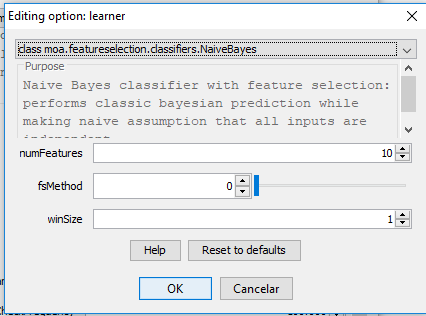
\includegraphics[width=.8\textwidth]{configuration_moa.png}
    \caption{Tela de configurações do MOA para execução dos experimentos.}
    \label{fig:configuracao_moa}
\end{figure}

Neste tela, o usuário possui três opções de configuração, descritas a seguir:

\begin{itemize}
\item \textit{numFeatures}: quantidade de atributos que o algoritmo de seleção de atributos deve selecionar ao fina de sua execução.
\item \textit{fsMethod}: algoritmo de seleção de atributos à ser avaliado. A opção 0, padrão, indica que nenhuma seleção de atributos será aplicada. Desse modo, o classificador utilizará todos os atributos contidos nos fluxos. A opção 1 é para utilização do Método de Katakis com Ganho de Informação. Opção 2 para utilização do FCBF e, por fim a opção 3 para utilização do algoritmo OFS.
\item \textit{winSize}: janela de processamento. Define quantos fluxos serão processados por vez. O padrão é 1.
\end{itemize}

\end{document}